% This file was converted to LaTeX by Writer2LaTeX ver. 1.6.1
% see http://writer2latex.sourceforge.net for more info
\documentclass[a4paper,12pt]{jarticle}
%\usepackage[utf8]{inputenc}
\usepackage{amsmath}
\usepackage{amssymb,amsfonts,textcomp}
%\usepackage[T1]{fontenc}
%\usepackage[english]{babel}
\usepackage{color}
\usepackage{array}
\usepackage{supertabular}
\usepackage{hhline}
\usepackage[dvipdfmx]{hyperref}
\usepackage{pxjahyper}
\usepackage{lastpage}
\hypersetup{colorlinks=true, linkcolor=blue, citecolor=blue, filecolor=blue, urlcolor=blue}
\usepackage[dvipdfmx]{graphicx}
\graphicspath{%
{./text01-img/}%
}
%\usepackage{svg}
\usepackage{bbding,pifont,wasysym,amssymb}
% Outline numbering
\setcounter{secnumdepth}{2}
\renewcommand\thesection{\arabic{section}}
\renewcommand\thesubsection{\arabic{section}.\arabic{subsection}}
\makeatletter
\newcommand\arraybslash{\let\\\@arraycr}
\makeatother
% Page layout (geometry)
\setlength\voffset{-1in}
\setlength\hoffset{-1in}
\setlength\topmargin{2cm}
\setlength\oddsidemargin{2cm}
\setlength\textheight{24.770668cm}
\setlength\textwidth{17.006cm}
\setlength\footskip{26.144882pt}
\setlength\headheight{0cm}
\setlength\headsep{0cm}
% Footnote rule
\setlength{\skip\footins}{0.12cm}
\renewcommand\footnoterule{\vspace*{-0.018cm}\setlength\leftskip{0pt}\setlength\rightskip{0pt plus 1fil}\noindent\textcolor{black}{\rule{0.25\columnwidth}{0.018cm}}\vspace*{0.102cm}}
% Pages styles
\makeatletter
\newcommand\ps@Standard{
  \renewcommand\@oddhead{}
  \renewcommand\@evenhead{}
  \renewcommand\@oddfoot{ \hspace{80mm} 子どもIT未来塾~~第1回 \hfill \thepage\ / \pageref{LastPage}}
  \renewcommand\@evenfoot{\@oddfoot}
  \renewcommand\thepage{\arabic{page}}
}
\newcommand\ps@FirstPage{
  \renewcommand\@oddhead{}
  \renewcommand\@evenhead{}
  \renewcommand\@oddfoot{}
  \renewcommand\@evenfoot{\@oddfoot}
  \renewcommand\thepage{\arabic{page}}
}
\makeatother
\pagestyle{Standard}
\setlength\tabcolsep{1mm}
\renewcommand\arraystretch{1.3}
% List styles
\newcounter{saveenum}
\newcounter{Figure}
\renewcommand\theFigure{\arabic{Figure}}
\title{\Huge\bf 子どもIT未来塾 第1回}
\author{
\huge\bf ラズベリーパイの使い方・\\
\huge\bf 自己紹介ページを作ろう\\
\vspace{15mm}
}
\date{ \Huge 清水 尚彦 先生 }
\begin{document}
\clearpage\setcounter{page}{1}\pagestyle{Standard}
\thispagestyle{FirstPage}

\maketitle

\setcounter{page}{1}\pagestyle{Standard}
\clearpage

\if00

\section{今回の授業}
\subsection{目標}
\ \ \ \ ラズベリーパイになれよう

\ \ \ \ 自分のホームページを作れるようになろう

\subsection{授業内容}
%\liststyleLii
\begin{enumerate}
\item ラズベリーパイとは
\item ラズベリーパイになれよう(1)
\item ラズベリーパイになれよう(2)
\item 自分の紹介ページを作ろう
\end{enumerate}
\subsection{注意点}
%\liststyleLiii
\begin{itemize}
\item
授業の合間のきゅうけいでは、遠くのものをながめたりして目を休めましょう
\item 水分ほきゅうはこまめにしましょう
\item
先生が説明中は先生の話を聞きましょう
\item
わからないことがあったらTAの先生方にすぐ聞きましょう
\end{itemize}
\subsection{教科書について}
%\liststyleLiv
\begin{itemize}
\item
教科書には例題、それに似た問題があります。まずは、例題をよく読みながら試してみましょう。そのあと問題を解きましょう。問題の答えは一番最後のページにあります。
\end{itemize}
\clearpage\subsection{配布物の確認}

\bigskip

%\liststyleLv
\begin{enumerate}
\item ラズベリーパイ
\item SDカード(16GB)
\item でんげんケーブル
\item HDMIケーブル
\item キーボード
\item ヘッドセット
\item マウス
\item センサーボード
\item ウェブカメラ
\item ディスプレイ(持って帰れません)
\end{enumerate}
\clearpage

\begin{tabular}{cc}
\includegraphics[width=6.488cm,height=4.697cm]{textbook-img009.png}
	&
\includegraphics[width=6.488cm,height=4.697cm]{textbook-img010.png} \\

\includegraphics[width=6.488cm,height=4.697cm]{textbook-img007.png}
	&
\includegraphics[width=6.488cm,height=4.697cm]{textbook-img008.png} \\

\includegraphics[width=6.488cm,height=4.697cm]{textbook-img005.png}
	&
\includegraphics[width=6.488cm,height=4.697cm]{textbook-img006.png} \\

\includegraphics[width=6.488cm,height=4.697cm]{textbook-img003.png}
	&
\includegraphics[width=6.488cm,height=4.697cm]{textbook-img004.png} \\

\includegraphics[width=6.488cm,height=4.697cm]{textbook-img002.png}
	&
\includegraphics[width=6.488cm,height=4.697cm]{textbook-img001.png} \\
\end{tabular}

%\liststyleLv
\subsection{ラズベリーパイについて}
イギリスのラズベリーパイ財団というグループが開発したカードと同じくらいの大きさのコンピュータです。ラズベリーパイは短くラズパイとも呼ばれています。

\subsection{とくちょう}
%\liststyleLvi
\begin{itemize}
\item 小さい( UNO 、トランプ、 Suica
などと同じ大きさ)
\item 普通のパソコンのように使える
\item (動画再生やゲームもできます)
\item
プログラミングのべんきょうに向いている
\item
モータやライトをせいぎょできる(目に見えるのでプログラミングを楽しめる)
\end{itemize}
\subsection{ラズベリーパイでできること}
プログラミングを手軽に学ぶことができます。プログラミングをするときにはパソコンが必要

でお金もかかりやりたくてもできないひともいたかもしれません。しかし、ラズベリーパイの

ような小さくて手に入れやすいコンピュータがあれば手軽にプログラミングの学習に取り組む

ことができます。また、ラズベリーパイを使うことでモータやライトなどを動かしたり光らせ

たりすることができます。これらのせいぎょをプログラムで行うことができるので楽しみなが

ら学習を進められます。

\subsection{ラズベリーパイを使うときの注意}
%\liststyleLvii
\begin{itemize}
\item
水などぬれているものをラズベリーパイ本体につけないようにしましょう
\end{itemize}
%\liststyleLviii
\begin{itemize}
\item
ラズベリーパイをはじめコンピュータなどは熱に弱いのですごく暑い部屋では使わないようにしましょう
\end{itemize}
%\liststyleLix
\begin{itemize}
\item
ラズベリーパイの本体をあまりさわらないようにしましょう
\item
ラズベリーパイなどは静電気によわいので注意しましょう
\end{itemize}
%\liststyleLx
\begin{itemize}
\item
ラズベリーパイをらんぼうに扱うのはやめましょう
\end{itemize}
%\liststyleLxi
\begin{itemize}
\item
金属のものの上におかないようにしましょう
\end{itemize}

\clearpage

\subsection{ラズベリーパイを準備しよう(手順)}
\ \ ラズベリーパイとキーボード、マウス等を接続して起動する準備をします。

\begin{figure}[ht]
\centering
\begin{minipage}{12.204cm}
{\upshape
\includegraphics[width=0.6\textwidth]{connections01.png}
 \newline
Figure \stepcounter{Figure}{\theFigure}: 接続のかんたんな図}

\end{minipage}
\end{figure}

%\liststyleLxii
\begin{enumerate}
\item ラズベリーパイとモニタをつなぐ

\begin{itemize}
\item
ラズベリーパイとモニタをHDMIケーブルで接続します。Figure~\ref{seq:refFigure1}、Figure~\ref{seq:refFigure2}を参考にしてください。お家でやる場合は、モニタもしくはTVによってはHDMIの差込口の場所が異なる場合があります。説明書等を別途参照してください\textbf{。}


		\begin{figure}[h]
			\begin{minipage}{0.5\textwidth}
{\upshape
  %[Warning: Image ignored] % Unhandled or unsupported graphics:
\includegraphics[width=5.519cm,height=4.471cm]{textbook-img015.png}
 \newline
Figure {\refstepcounter{Figure}\theFigure\label{seq:refFigure1}}:
ラズベリーパイHDMI接続}
			\end{minipage}
			\begin{minipage}{0.5\textwidth}
{\upshape
  %[Warning: Image ignored] % Unhandled or unsupported graphics:
\includegraphics[width=5.519cm,height=4.471cm]{textbook-img016.png}
 \newline
Figure {\refstepcounter{Figure}\theFigure\label{seq:refFigure2}}:
ディスプレイHDMI接続}
			\end{minipage}
\end{figure}

\end{itemize}
\item マウスとキーボードをつなぐ

\begin{itemize}
\item
マウス、キーボードの先をラズベリーパイへ差し込みます。
\end{itemize}
\end{enumerate}

\begin{figure}[h]
\begin{minipage}{8.135cm}
{\upshape
\includegraphics[width=8.135cm]{textbook-img017.png}
 \newline
Figure \stepcounter{Figure}{\theFigure}:
マウス、キーボードの接続}
\end{minipage}
\end{figure}
%\liststyleLxii
\setcounter{saveenum}{\value{enumi}}
\begin{enumerate}
\setcounter{enumi}{\value{saveenum}}
	\clearpage
\item
microSD(マイクロエスディー)
カードをいれる

\begin{itemize}
\item
	microSDカードをラズベリーパイ本体(ウラ面)にさします。小さいのでなくさないように気をつけましょう。

\begin{figure}[h]
\centering
\begin{minipage}{6.334cm}
{\upshape
\includegraphics[width=5.292cm,height=3.545cm]{textbook-img018.png}
 \newline
Figure \stepcounter{Figure}{\theFigure}: microSDカードのさしこみ}
\end{minipage}
\end{figure}

\bigskip
\end{itemize}
\item モニタのでんげんをいれる

\begin{itemize}
\item
次にモニタのコンセントをさします。モニタのみぎはじのボタンをおします。でんげんが入ると青色にてんとうします。お家でやるときはでんげんのいれた後、入力きりかえが必要となる場合がありますので、説明書等を別途参照してください。


\begin{figure}[h]
\centering
\begin{minipage}{6.172cm}
{\upshape
\includegraphics[width=6.318cm,height=4.685cm]{textbook-img019.png}
 \newline
Figure \stepcounter{Figure}{\theFigure}:
モニタでんげんボタンの位置}
\end{minipage}
\end{figure}
\end{itemize}
\item ラズベリーパイのでんげんをいれる

\begin{itemize}
\item
最後にラズベリーパイのでんげんをいれます。Figure~\ref{seq:refFigure6}のようにラズベリーパイにでんげんケーブルをさしてコンセントへ接続します。赤色のランプがついてディスプレイにラズベリーが表示がされますFigure~\ref{seq:refFigure7}。Figure~\ref{seq:refFigure8}のような画面になったら起動は完了です。
\end{itemize}
\begin{figure}
\centering
\begin{minipage}{5.228cm}
{\upshape
\includegraphics[width=4.613cm,height=3.856cm]{textbook-img020.png}
 \newline
Figure {\refstepcounter{Figure}\theFigure\label{seq:refFigure6}}:
ラズベリーパイでんげん接続}
\end{minipage}
\begin{minipage}{5.371cm}
{\upshape
\includegraphics[width=4.782cm,height=3.919cm]{textbook-img021.png}
 \newline
Figure {\refstepcounter{Figure}\theFigure\label{seq:refFigure7}}:
ラズベリーパイ起動中}
\end{minipage}
\begin{minipage}{4.724cm}
{\upshape
\includegraphics[width=4.724cm,height=3.314cm]{textbook-img022.png}
 \newline
Figure {\refstepcounter{Figure}\theFigure\label{seq:refFigure8}}: 起動時画面}
\end{minipage}
\end{figure}
\item インターネットに接続\\
\ \ まずは画面右上のほうにあるWi-Fiのアイコンをクリックします。Figure~\ref{seq:refFigure10}の赤わくで囲われています。クリックするとFigure~\ref{seq:refFigure9}のようにWi-Fiのいちらんが出てきます。接続するアクセスポイントを選びます。

\end{enumerate}


\begin{figure}[h]
\centering
\begin{minipage}{6.597cm}
{\upshape
\includegraphics[width=4.068cm,height=4.987cm]{textbook-img024.png}
 \newline
Figure {\refstepcounter{Figure}\theFigure\label{seq:refFigure10}}: Wi-Fi接続メニュー}
\end{minipage}
\begin{minipage}{5.957cm}
{\upshape
\includegraphics[width=3.427cm,height=4.738cm]{textbook-img023.png}
 \newline
Figure {\refstepcounter{Figure}\theFigure\label{seq:refFigure9}}: SSIDいちらん}
\end{minipage}
\end{figure}
にんしょうが必要なアクセスポイントの場合は、パスワードの入力を求められます。赤わくの中にパスワードを入力してOKを押します。

\begin{figure}
\centering
\begin{minipage}{7.712cm}
{\upshape
\includegraphics[width=7.712cm,height=3.888cm]{textbook-img026.png}
 \newline
Figure \stepcounter{Figure}{\theFigure}: パスワード入力画面}
\end{minipage}
\begin{minipage}{7.241cm}
{\upshape
\includegraphics[width=5.577cm,height=3.228cm]{textbook-img025.png}
 \newline
Figure \stepcounter{Figure}{\theFigure}: パスワード入力画面}
\end{minipage}
\end{figure}
問題なく接続ができれば、Wi-FiのアイコンがFigure~\ref{seq:refFigure13}のようになります。これで接続は完了です。お家でやるときは、Wi-Fiのルーター等の説明書等を参照してください。

\begin{figure}
\centering
\begin{minipage}{7.334cm}
{\upshape
\includegraphics[width=5.708cm,height=3.895cm]{textbook-img027.png}
 \newline
Figure {\refstepcounter{Figure}\theFigure\label{seq:refFigure13}}:
接続後のアイコン}
\end{minipage}
\end{figure}
\clearpage\section{ラズベリーパイになれよう(1)}
\subsection{ファイル、フォルダ}
\ \ コンピュータやラズベリーパイの中にあるデータ(音楽、動画、写真、テキストなど)はすべてファイルとして扱われています。しばしばファイルには.(ドット)から始まる「拡張子」がついており、ファイルがどんな種類なのかを表します。例えば画像の場合は.jpgや動画ファイルの場合はmp4、テキストファイルは.txt、ホームページの場合は.htmlがついています。

ファイルの他にフォルダというものがあります。フォルダはファイルをまとめたものです。ファイルを書類としてフォルダはバインダと考えるとわかりやすいでしょう。フォルダのなかにフォルダをいれることもできます。



\begin{figure}[hb]
\centering
\begin{minipage}{13.148cm}


\includegraphics[width=13.148cm]{figure15.png}
{\upshape
\newline
Figure \stepcounter{Figure}{\theFigure}:
フォルダ、ファイルの関係}
\end{minipage}
\end{figure}

	\begin{minipage}{\textwidth}
\begin{minipage}{5.562cm}
	\centering
\textbf{(左)クリック}
\flushleft

	カチッ\\
	\centering
\raisebox{20mm}{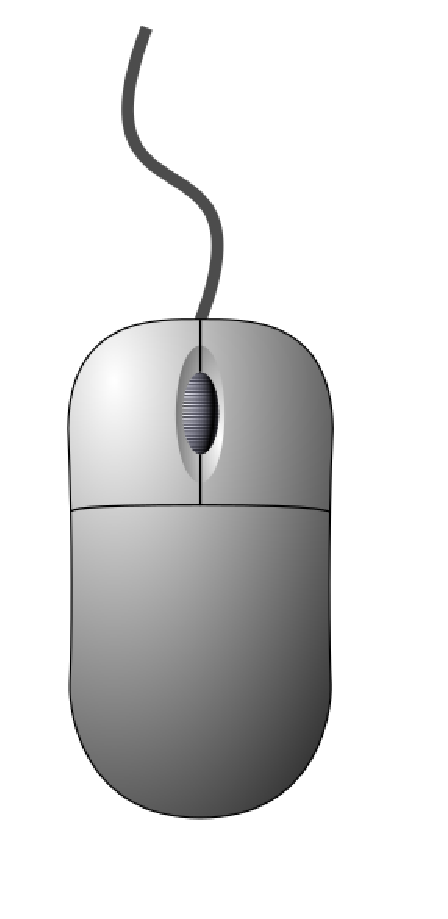
\includegraphics[width=1.651cm,height=3.53cm]{textbook-img076.eps}}

\flushleft
マウスの左側を一度押すこと、アプリなど開きたいときに使おう
\end{minipage}
\begin{minipage}{5.562cm}
	\centering
\textbf{ダブルクリック}
\flushleft

	カチカチッ\\
\centering
\raisebox{20mm}{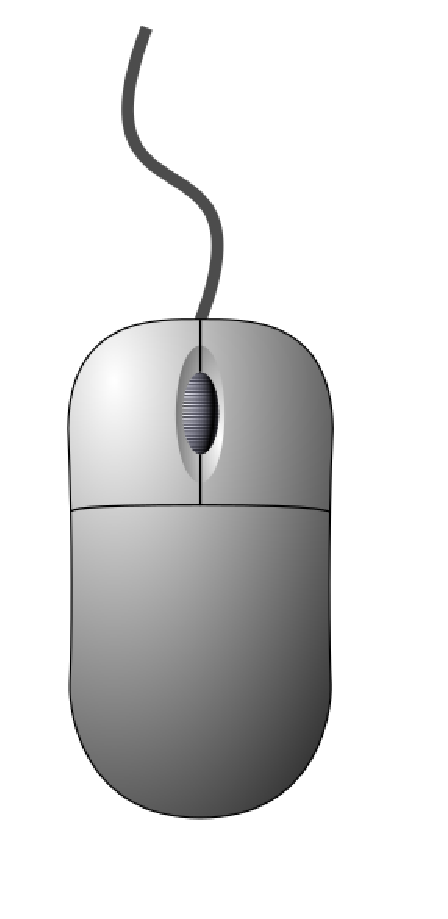
\includegraphics[width=1.651cm,height=3.53cm]{textbook-img076.eps}}


\flushleft
マウスの左側を二回続けて押すこと。 デスクトップのフォルダなどを開くときに使うよ
\end{minipage}
\begin{minipage}{5.562cm}
	\centering
\textbf{~~~~~右クリック}
\flushleft

	\hspace{3cm} カチッ\\
	\centering
\raisebox{20mm}{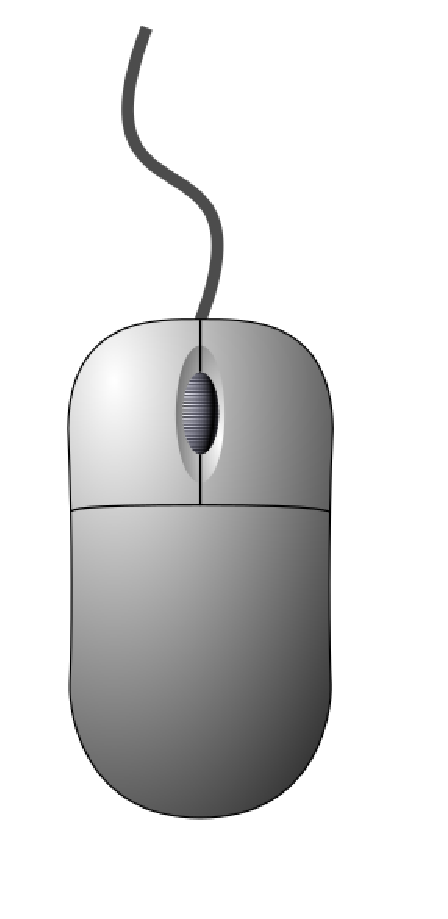
\includegraphics[width=1.651cm,height=3.53cm]{textbook-img076.eps}}


\flushleft
マウスの右側を一度押すこと。メニューなどを表示したいときに使うよ
\end{minipage}
\end{minipage}


\clearpage

\subsection{例題 1-1フォルダを作成しよう}
自身のフォルダを開き、Documentsフォルダ直下にtaro、hanako、saburoという名前のフォルダを作成しよう\\

{\bf \large 考え方}
\vfill
\begin{figure}[ht]
	\begin{minipage}{\textwidth}
%[Warning: Image ignored] % Unhandled or unsupported graphics:
\includegraphics[width=6.472cm,height=4.976cm]{textbook-img032.png}
\includegraphics[width=2.094cm,height=1.771cm]{textbook-img035.png}
\includegraphics[width=8.301cm,height=4.948cm]{textbook-img033.png}
	\end{minipage}
\begin{minipage}{0.4\textwidth}
1
ディスプレイの左上の アイコンをクリック
\end{minipage}
\hfill
\begin{minipage}{0.4\textwidth}
2
上の図にファイルマネージャーが表示されます
\end{minipage}\\
	\vspace{-12mm}
	\hfill \includegraphics[width=1.771cm,height=2.094cm]{textbook-img037.png}
	%\vspace{-5mm}
\includegraphics[width=0.9\textwidth]{textbook-img034.png}
\begin{minipage}{15.758cm}
\centering
3
右側の空白部分で右クリックし 新規作成からフォルダを選んでクリック
\end{minipage}
\begin{minipage}{\textwidth}
\includegraphics[width=0.9\textwidth]{textbook-img036.png}
\end{minipage}
\begin{minipage}{12.336cm}
4
フォルダ名の入力を求められるので、付けたい名前を入力しよう
\end{minipage}
\end{figure}
\clearpage
{\bf\large 考え方(続き)}



\begin{figure}[hb]
\centering
%[Warning: Image ignored] % Unhandled or unsupported graphics:
\includegraphics[width=11.398cm,height=5.72cm]{textbook-img038.png}
\centering
\begin{minipage}{13.001cm}
5
名前を入力し、OKを押すと上の画像のようにフォルダが作成されます
\end{minipage}

\end{figure}
\begin{figure}[hb]
\centering
\begin{minipage}{0.8\textwidth}
	{	\large
フォルダは大事です。

フォルダに、画像やプログラムのコードを保存しておくので、わかりやすく関係性のある名前を付けてあげましょう

\bigskip
ファイルやフォルダの名前は、
空白の入らない半角ローマ字にしておくと、
後でプログラムから使う時に便利だよ
	}
\end{minipage}
\end{figure}
\clearpage
\begin{figure}[ht]
\flushleft{\bf\large 答え}
	\vspace{8mm}\\
\centering
\includegraphics[width=13.33cm,height=4.74cm]{textbook-img034.png}
\begin{minipage}{\textwidth}
1
左上のフォルダアイコンをクリックし

 フォルダマネージャー上で右クリックし、上の画像のようにしよう
\end{minipage}

\centering
%[Warning: Image ignored] % Unhandled or unsupported graphics:
\includegraphics[width=12.483cm,height=4.584cm]{textbook-img036.png}
\begin{minipage}{\textwidth}
2
\ 新規作成のところからフォルダを選び、名前設定に行こう
\end{minipage}

\centering
%[Warning: Image ignored] % Unhandled or unsupported graphics:
\includegraphics[width=12.776cm,height=3.879cm]{textbook-img039.png}
\begin{minipage}{\textwidth}
3 taroと名前を入力し、OKを押す
\end{minipage}

\centering
%[Warning: Image ignored] % Unhandled or unsupported graphics:
\includegraphics[width=12.659cm,height=3.972cm]{textbook-img040.png}
\begin{minipage}{\textwidth}
4 taroというフォルダを作成できていることを確認しよう
\end{minipage}

\end{figure}
\clearpage
\begin{figure}
	\flushleft{\bf\large
	答え(続き)}\\
	\vspace{10mm}
\centering
%[Warning: Image ignored] % Unhandled or unsupported graphics:
\includegraphics[width=14.289cm,height=5.431cm]{textbook-img041.png}
\begin{minipage}{\textwidth}
\ 5
\ 先ほどと同じように右クリックから新規作成、フォルダを選び、hanakoという名前でフォルダを作成
\end{minipage}

\centering
%[Warning: Image ignored] % Unhandled or unsupported graphics:
\includegraphics[width=13.884cm,height=4.189cm]{textbook-img042.png}
\begin{minipage}{\textwidth}
\ 6
\ saburoというフォルダを先ほどと同じ方法で作成
\end{minipage}

\centering
%[Warning: Image ignored] % Unhandled or unsupported graphics:
\includegraphics[width=8.359cm,height=4.761cm]{textbook-img043.png}
\begin{minipage}{\textwidth}
\ 7 \ taro , hanako ,
saburoのフォルダが作成されていることを確認してみよう
\end{minipage}
	\vspace{10mm}
\flushleft
{\bfseries
問題 1-1}

 例題と同じ方法で、akahoshi、imaoka、hamanakaという名前のフォルダを作ろう

\end{figure}
\clearpage\subsection{例題 1-2フォルダを移動しよう}
Desktop直下に「space1」と「space2」を作り、「space1」の中に「move」フォルダを作り、「move」フォルダを「space2」に移動しよう

\flushleft{\bf\large 考え方}


\begin{figure}[ht]
\centering
%[Warning: Image ignored] % Unhandled or unsupported graphics:
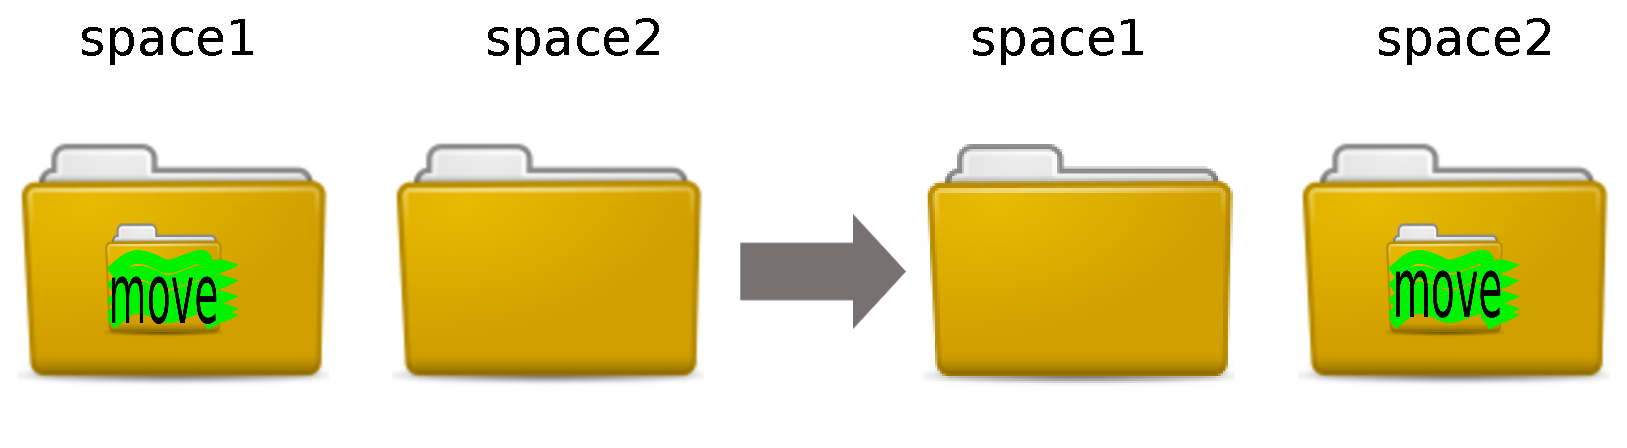
\includegraphics[width=0.8\textwidth]{fig15-1.eps}
\begin{minipage}{15.297cm}
フォルダやファイルは後からでも動かすことができるよ。
\end{minipage}

\begin{minipage}{5.963cm}
\includegraphics[width=3.604cm,height=2.268cm]{textbook-img051.png}
	{\flushleft
1
左側のDesktopをクリック しspace1とspace2を作成
	}
\end{minipage}
\includegraphics[width=2.168cm,height=1.542cm]{textbook-img052.png}
\begin{minipage}{7.473cm}
\includegraphics[width=5.166cm,height=1.882cm]{textbook-img050.png}
	{\flushleft
2 space1の中にmoveフォルダを作成
	}
\end{minipage}

\centering
\begin{minipage}{6.589cm}
\includegraphics[width=3.584cm,height=3.658cm]{textbook-img048.png}
	{\flushleft
3
moveフォルダ上で右クリックし、 切り取りをクリック
	}
\end{minipage}
\includegraphics[width=2.168cm,height=1.542cm]{textbook-img049.png}
\begin{minipage}{6.589cm}
%\includegraphics[width=2.168cm,height=1.542cm]{textbook-img047.png}
\includegraphics[width=5.225cm,height=4.119cm]{textbook-img046.png}
	{\flushleft
4
space2の中で右クリック、貼り付けをクリック
	}
\end{minipage}

%[Warning: Image ignored] % Unhandled or unsupported graphics:
\begin{minipage}{6.589cm}
\includegraphics[width=7.218cm,height=3.281cm]{textbook-img045.png}
	{\flushleft
5
space1の中にあったmoveフォルダがspace2に移動しました
	}
\end{minipage}


\end{figure}


{\bfseries 問題 1-2}
「space1」フォルダ内に「rasp」フォルダを作り、さらにそのフォルダ内に「berry」フォルダを作成して「rasp」フォルダを「space2」フォルダに移動させよう。そして中身を確認しよう



\clearpage\subsection{例題 1-3ファイル名を変更しよう}
「before」という名前のフォルダをDocuments直下に1つ作り、その作成した後でフォルダ名を「after」に変えよう

\begin{figure}[ht]
\flushleft{\bf\large 考え方}

\centering
%[Warning: Image ignored] % Unhandled or unsupported graphics:
\begin{minipage}{1.978cm}
\includegraphics[width=1.45cm,height=1.45cm]{textbook-img044.png}
frog
\end{minipage}
\includegraphics[width=2.168cm,height=1.542cm]{textbook-img052.png}
\begin{minipage}{1.978cm}
\includegraphics[width=1.588cm,height=1.588cm]{textbook-img044.png}
dog
\end{minipage}
\begin{minipage}{6.319cm}
まちがったフォルダ名をつけたとき、名前を変えたいときなど
に使います。
\end{minipage}

\begin{minipage}{6.656cm}
\includegraphics[width=6.96cm,height=4.824cm]{textbook-img058.png}
\flushleft
1
左側のDocumentsをクリックし「before」フォルダを作成
\end{minipage}
\includegraphics[width=2.168cm,height=1.542cm]{textbook-img052.png}
\begin{minipage}{5.751cm}
\includegraphics[width=6.555cm,height=5.941cm]{textbook-img057.png}
\flushleft
2 フォルダ上で右クリックし、

 ファイル名の変更をクリック
\end{minipage}
%[Warning: Image ignored] % Unhandled or unsupported graphics:

\begin{minipage}{6.973cm}
\includegraphics[width=6.973cm,height=5.327cm]{textbook-img055.png}
3 名前を「after」に変更

 OKをクリック
\end{minipage}
\includegraphics[width=1.919cm,height=1.365cm]{textbook-img053.png}
\begin{minipage}{5.751cm}
\includegraphics[width=5.92cm,height=4.51cm]{textbook-img056.png}
4 変更を確認
\end{minipage}
\centering

\begin{minipage}{5.751cm}
フォルダ名の変更は、よく使うので覚えておこう
\end{minipage}
\end{figure}


{\bfseries
問題 1-3}

「miss\_name」という名前のフォルダを1つ作り、その作成した後でフォルダ名を「success\_name」に変えよう

\clearpage
\begin{figure}[ht]
\subsection{例題 1-4
日本語入力と英字入力について}
\ Text
Editorを開き、アルファベットをa〜zまで入力しよう。その後「こんにちは」「こんばんは」「ごきげんよう」「さようなら」「ありがとう」をそれぞれ一行に入力しましょう。

{\bf\large 考え方}


\centering
	\begin{minipage}{\textwidth}
\includegraphics[width=7.459cm,height=2.245cm]{textbook-img065.png}
		\raisebox{10mm}
		{
\begin{minipage}{0.5\textwidth}
赤わくで囲んだ
Ctrlとスペースを
同時に押すことで
英字入力と日本語入力を
切り替えることができるよ
\end{minipage}
}
\end{minipage}

\begin{minipage}{6.984cm}
\includegraphics[width=5.408cm,height=5.595cm]{textbook-img064.png}
\flushleft
1
ラズベリーのアイコンをクリックしてアクセサリー>Text
editorを開こう
\end{minipage}
\includegraphics[width=1.919cm,height=1.365cm]{textbook-img053.png}
\begin{minipage}{7.347cm}
\includegraphics[width=7.897cm,height=3.655cm]{textbook-img063.png}
\flushleft
2.
赤線が引かれているところをクリックしてテキストエディタにカーソル(縦棒)が入っていることを確認してください。
\end{minipage}

\begin{minipage}{7.238cm}
\includegraphics[width=6.643cm,height=2.533cm]{textbook-img059.png}
\flushleft
3. Ctrlとスペースキーを同時に押して 

 英字入力に切り替えよう。アイコンがキーボードであることを確認しよう。
\end{minipage}
\includegraphics[width=1.919cm,height=1.365cm]{textbook-img053.png}
\begin{minipage}{7.351cm}
\includegraphics[width=6.514cm,height=2.856cm]{textbook-img061.png}
\flushleft
4. 英字入力でa〜zまで入力しよう
\end{minipage}

\begin{minipage}{6.73cm}
\includegraphics[width=4.029cm,height=2.586cm]{textbook-img062.png}
\flushleft
5. Ctrlとスペースキーを同時に押して
アイコンが“あ”になったか確認しましょう。
\end{minipage}
\includegraphics[width=1.919cm,height=1.365cm]{textbook-img053.png}
\begin{minipage}{6.589cm}
\includegraphics[width=4.914cm,height=3.616cm]{textbook-img060.png}
\flushleft
6. こんにちは〜ありがとうを入力\\
7. 完成
\end{minipage}



\flushleft
{\bfseries 問題 1-4}
Text editorでA〜Zを入力しよう 

ヒント 

英字入力時にshiftキーを押しながらアルファベットキーを打つと大文字で入力できます
\end{figure}
\clearpage
\begin{figure}[ht]
\subsection{例題
1-5半角入力と全角入力について}
Text
Editorを開き、半角入力でアルファベットをa〜zまで入力し、その後、全角入力で

アルファベットa〜zまで入力しよう。全角と半角文字の違いを理解しよう。

{\bf\large 考え方}

\centering
%[Warning: Image ignored] % Unhandled or unsupported graphics:
\includegraphics[width=5.978cm,height=1.773cm]{textbook-img066.png}
	\raisebox{8mm}{
\begin{minipage}{6.762cm}
{文字が小さいのが半角}\\
{文字が大きいのが全角}
\end{minipage}
}

\begin{minipage}{16.578cm}

\bigskip

アルファベットのサイズからも分かる通り、大きいサイズが全角で、小さいサイズが半角だと覚えておくといいよ
\end{minipage}
%[Warning: Image ignored] % Unhandled or unsupported graphics:
\begin{minipage}{5.578cm}
\includegraphics[width=5.172cm,height=3.924cm]{textbook-img067.png}
\flushleft
1 Text editorを開こう
\end{minipage}
\includegraphics[width=1.919cm,height=1.365cm]{textbook-img053.png}
\begin{minipage}{7.931cm}
\includegraphics[width=7.868cm,height=2.534cm]{textbook-img059.png}
\flushleft
2
キーボードのアイコンになっていることを確認して半角を入力しよう
\end{minipage}
\begin{minipage}{6.345cm}
\includegraphics[width=4.889cm,height=2.596cm]{textbook-img059.png}
\flushleft
3
半角のアルファベットを入力し終えたら右上のキーボードアイコンをクリック
\end{minipage}
\includegraphics[width=1.919cm,height=1.365cm]{textbook-img053.png}
\begin{minipage}{7.524cm}
\includegraphics[width=5.471cm,height=2.469cm]{textbook-img062.png}
\flushleft
4
アイコンが変わったことを確認しよう
\end{minipage}

\begin{minipage}{7.173cm}
\includegraphics[width=5.889cm,height=3.596cm]{textbook-img069.png}
\flushleft
5 アイコンを右クリックして、

全角英数を選択
\end{minipage}
\includegraphics[width=1.919cm,height=1.365cm]{textbook-img053.png}
\begin{minipage}{7.178cm}
\includegraphics[width=7.471cm,height=3.469cm]{textbook-img070.png}
\flushleft
6 入力
\end{minipage}

\vspace{3mm}
\begin{minipage}{16.578cm}
{\centering\large
プログラミングでアルファベット,記号を入力するときは
半角(小さい文字)で入力しましょう
}
\end{minipage}

\flushleft
{\bfseries 問題 1-5}

Text editorで半角A〜Zと全角A〜Zを入力しよう 

ヒント


英字入力時にshiftキーを押しながらアルファベットキーを打つと大文字で入力できます
\end{figure}
\clearpage
\begin{figure}[t]
\subsection{ブラウザでけんさくをしよう}
ブラウザを開いてけんさくをしよう。ブラウザを使用するとウェブサイトを開くことができます。もし、困ったことがあったら自分でけんさくをできるように使い方を覚えておきましょう。

\subsection{例題 1-6
ブラウザ立ち上げとマウスそうさについて}
ブラウザを立ち上げ、好きなものを調べよう

{\bf\large 考え方}

	\begin{minipage}{\textwidth}
\begin{minipage}{6.204cm}
\includegraphics[width=5.426cm,height=2.849cm]{textbook-img071.png}
1,デスクトップの左上のアイコンを左クリック
\end{minipage}
\includegraphics[width=1.505cm,height=1.707cm]{textbook-img073.png}
\begin{minipage}{8.233cm}
\includegraphics[width=8.373cm,height=3.193cm]{textbook-img075.png}
2,
ブラウザが立ち上がり、赤で囲われている部分を左クリック
\end{minipage}
	\end{minipage}

\hfill\begin{minipage}{7.78cm}
	{\centering
\includegraphics[width=1.707cm,height=1.505cm]{textbook-img074.png}
	}\\
\includegraphics[width=7.742cm,height=3.771cm]{textbook-img072.png}
3,
キーボードでけんさくしたいワード を入力しよう。入力し終えたらenterキーを押そう
\end{minipage}

	\vspace{70mm}

\end{figure}
\clearpage
\begin{figure}
Figure~\ref{seq:refFigure15}のように赤い四角で囲われているところにけんさくしたい言葉を入れてエンターキーを押すとけんさくができます。例えば”ねこ”とけんさくしてみましょう。
	\centering
{\upshape
\includegraphics[width=12.023cm,height=4.447cm]{textbook-img077.png}

Figure{\refstepcounter{Figure}\theFigure\label{seq:refFigure15}}: けんさくバー}


	\flushleft
けんさくするとFigure~\ref{seq:refFigure16}このような感じになります。青線で囲んであるところは今けんさくした言葉です。赤線で囲われている\textbf{画像}をクリックすると画像をけんさくできます。クリックしてみましょう。
	

	\centering
{\upshape
\includegraphics[width=12.123cm,height=4.299cm]{textbook-img078.png}
 \newline
Figure {\refstepcounter{Figure}\theFigure\label{seq:refFigure16}}:
”ねこ”けんさく結果\\
けんりの関けいで画像をぼかしてあります}

	\flushleft
Figure~\ref{seq:refFigure17}のように”ねこ”の画像がたくさんでてきました。けんさくしたい言葉のけんさく結果を画像できました。\textbf{Web}をクリックすると先ほどのFigure~\ref{seq:refFigure16}のようなホームページけんさくに戻れます。


\centering
\begin{minipage}{13.762cm}
\includegraphics[width=13.892cm,height=5.156cm]{textbook-img079.png}

Figure {\refstepcounter{Figure}\theFigure\label{seq:refFigure17}}:
”ねこ”画像けんさく結果
\end{minipage}

\flushleft
{\bfseries
問題 1-6}

\ \ 自分の好きなキーワードをけんさくしてみよう

\end{figure}
\clearpage
\begin{figure}[t]
\subsection{例題 1-7
キーボード入力の練習をしよう}
ブラウザで”
Etyping”とけんさくし、キーボードタイピングサイトでタイピングに慣れよう

\textbf{考え方}

\textbf{タイピング}\ \ ・・・キーボードで文字を入力すること\ \       
	\begin{minipage}{\textwidth}
		\raisebox{30mm}{		\begin{minipage}{0.65\textwidth}
パソコンでの文字入力はローマ字入力が基本です。
けんさくなどをしたいとき、キーボードで文字を入力します。
今回はタイピング練習サイト”Etyping”でタイピングを
練習しましょう。

\includegraphics[width=8.087cm,height=2.676cm]{textbook-img081.png}
\includegraphics[width=2.546cm,height=2.509cm]{textbook-img082.png}
		\end{minipage} }
\includegraphics[width=4.928cm,height=6.003cm]{textbook-img080.png}
	\end{minipage}

\centering


{\centering
\textbf{まずはタイピングゲームを開こう}
\par}

\centering

\begin{minipage}{5.695cm}
\includegraphics[width=5.523cm,height=4.249cm]{textbook-img071.png}
1 左上のアイコンをクリックしよう
\end{minipage}
\includegraphics[width=2.094cm,height=1.771cm]{textbook-img084.png}
\begin{minipage}{6.582cm}
\includegraphics[width=6.985cm,height=4.479cm]{textbook-img083.png}
2 けんさくらんに”Etyping”と入力しenterを押そう
\end{minipage}


\begin{minipage}{6.582cm}
\includegraphics[width=6.796cm,height=7.029cm]{textbook-img086.png}
3 サイトに入りましょう。赤わくで囲われているところをクリックします。
\end{minipage}
\begin{minipage}{8.482cm}
\includegraphics[width=8.714cm,height=2.163cm]{textbook-img085.png}
赤線で線が引かれているところ、黒い四角で囲んであるアイコンをよく確かめてください。
\end{minipage}






\centering



\end{figure}
\clearpage

\begin{figure}
\textbf{考え方(続き)}



\centering

\includegraphics[width=12.294cm,height=8.091cm]{textbook-img087.png}


\begin{minipage}{4.252cm}
4 ホームページが開けたら
黒で囲んである

\textbf{今すぐチェック!}

をクリックしよう

\end{minipage}
\end{figure}





\begin{figure}
\centering
\includegraphics[width=12.162cm,height=8.005cm]{textbook-img088.png}

\begin{minipage}{4.252cm}
5 黒い四角で囲んである

\textbf{今すぐチェック!}

をもう一度クリックします。
\end{minipage}
\end{figure}

\clearpage
\begin{figure}[t]
\subsection{ 考え方(続き)}

\centering
\includegraphics[width=9.719cm,height=6.396cm]{textbook-img091.png}
	\raisebox{40mm}{\begin{minipage}{4.252cm}
6 黒い四角で囲んである

\textbf{スタート}

をクリックします。
\end{minipage}
	}

\bigskip
\includegraphics[width=9.786cm,height=6.442cm]{textbook-img090.png}
	\raisebox{40mm}{\begin{minipage}{4.88cm}
7 キーボードのスペースキー

を押すとゲームがスタートします


\bigskip
\end{minipage}
	}

\bigskip


\bigskip

\includegraphics[width=9.895cm,height=6.512cm]{textbook-img089.png}
	\raisebox{30mm}{\begin{minipage}{4.88cm}
8 ゲームでは黒で囲んである文字をキーボードで入力します。


\bigskip

キーの位置は画面にオレンジで色がついています。


\bigskip

慣れてきたら、オレンジになっている指でキーボードを押せるように練習してみましょう。


\bigskip
\end{minipage}
	}

\bigskip
\bigskip
\bigskip
\bigskip
\end{figure}
\clearpage
\begin{figure}[t]
\subsection{例題 1-8
画像けんさくし、画像を保存しよう}
Documentsフォルダに自分の名前のフォルダを作り、さらにその中にkuma、usagi、inuフォルダを作成、そのフォルダに画像けんさくで得たクマ、うさぎ、犬の画像をそれぞれ対応するフォルダに保存しよう

\textbf{考え方}


\bigskip




	\centering
	\begin{minipage}{\textwidth}
\begin{minipage}{5.582cm}
\includegraphics[width=5.413cm,height=5.461cm]{textbook-img092.png}
\end{minipage}
\begin{minipage}{3.582cm}
	\includegraphics[width=1.505cm,height=1.707cm]{textbook-img073.png}
\end{minipage}
\begin{minipage}{5.582cm}
	\includegraphics[width=3.387cm,height=3.387cm]{textbook-img044.png}
\end{minipage}
	\end{minipage}


\flushleft
{\bfseries
フォルダに画像を保存しよう}

ブラウザの画像けんさくしたいものはラズベリーパイのフォルダ内に保存することができる

画像と関連のあるフォルダ名にしておくと、どのような画像が保存されているのかわかりやすいよ



	\begin{minipage}{\textwidth}
\begin{minipage}{6.582cm}
\includegraphics[width=5.401cm,height=4.152cm]{textbook-img093.png}\\
1 例題の方法で自分の名前のフォルダをDocuments内に作成しよう
\end{minipage}
\begin{minipage}{3.582cm}
	\raisebox{25mm}{\includegraphics[width=1.505cm,height=1.707cm]{textbook-img073.png}}
\end{minipage}
\begin{minipage}{6.582cm}
\includegraphics[width=5.995cm,height=3.475cm]{textbook-img094.jpg}\\
2 自分のフォルダをダブルクリックし、その中に上の画像のように3つのフォルダを作成
\end{minipage}
	\end{minipage}


	\begin{minipage}{\textwidth}
\begin{minipage}{7.033cm}
\includegraphics[width=7.049cm,height=5.554cm]{textbook-img096.png}\\
3 ブラウザを立ち上げてくまをけんさくし、上の画像の赤色で囲われた”画像”をクリック
\end{minipage}
\begin{minipage}{3.582cm}
	\raisebox{25mm}{\includegraphics[width=1.505cm,height=1.707cm]{textbook-img073.png}}
\end{minipage}
\begin{minipage}{6.582cm}
\includegraphics[width=6.468cm,height=5.406cm]{textbook-img095.png}\\
4 画像けんさくで好きな画像上で右クリックをし”名前をつけて保存”をクリック
\end{minipage}
	\end{minipage}


\end{figure}




\clearpage
\begin{figure}[t]
\textbf{考え方(続き)}



\centering
\begin{minipage}{\textwidth}
\begin{minipage}{7.289cm}
\includegraphics[width=6.8cm,height=3.48cm]{textbook-img097.png}\\
5 \ 名前を変更
\end{minipage}
\begin{minipage}{1.582cm}
	\raisebox{25mm}{\includegraphics[width=1.505cm,height=1.707cm]{textbook-img073.png}}
\end{minipage}
\begin{minipage}{6.582cm}
\includegraphics[width=8.375cm,height=2.448cm]{textbook-img098.png}\\
6 \ 自分の名前フォルダをダブルクリック
\end{minipage}
\end{minipage}


\bigskip

\begin{minipage}{\textwidth}
\begin{minipage}{6.582cm}
\includegraphics[width=6.671cm,height=2.314cm]{textbook-img100.png}\\
7 \ “kuma”フォルダをダブルクリック
\end{minipage}
\begin{minipage}{2.582cm}
	\raisebox{25mm}{\includegraphics[width=1.505cm,height=1.707cm]{textbook-img073.png}}
\end{minipage}
\begin{minipage}{6.582cm}
\includegraphics[width=7.668cm,height=4.023cm]{textbook-img099.png}\\
8 \ 名前と保存場所が決まったら右下の保存をクリック
\end{minipage}
\end{minipage}


\bigskip


\begin{minipage}{\textwidth}
\begin{minipage}{7.882cm}
\includegraphics[width=7.872cm,height=3.54cm]{textbook-img102.png}\\
9 \ kumaフォルダを開き、画像が保存されているか、確認しよう
\end{minipage}
\begin{minipage}{2.582cm}
	\raisebox{25mm}{\includegraphics[width=1.505cm,height=1.707cm]{textbook-img073.png}}
\end{minipage}
\begin{minipage}{6.582cm}
\includegraphics[width=6.71cm,height=4.228cm]{textbook-img101.png}\\
10 うさぎで検索し好きな画像を保存しよう
\end{minipage}
\end{minipage}

	\vspace{60mm}

\end{figure}



\bigskip



\clearpage

\begin{figure}[t]
\textbf{考え方(続き)}



\centering
\begin{minipage}{\textwidth}
\begin{minipage}{7.882cm}
\includegraphics[width=7.811cm,height=4.053cm]{textbook-img103.png}\\
11 \ 同じように保存フォルダと名前を決めて保存しよう
\end{minipage}
\begin{minipage}{2.582cm}
	\raisebox{25mm}{\includegraphics[width=1.505cm,height=1.707cm]{textbook-img073.png}}
\end{minipage}
\begin{minipage}{6.257cm}
\includegraphics[width=6.041cm,height=6.094cm]{textbook-img092.png}\\
12 \ 犬も同様
\end{minipage}
\end{minipage}


\bigskip


\begin{minipage}{\textwidth}
\begin{minipage}{7.22cm}
\includegraphics[width=6.911cm,height=3.729cm]{textbook-img105.png}\\
13 犬も同様
\end{minipage}
\begin{minipage}{2.582cm}
	\raisebox{25mm}{\includegraphics[width=1.505cm,height=1.707cm]{textbook-img073.png}}
\end{minipage}
\begin{minipage}{7.665cm}
\includegraphics[width=7.527cm,height=3.905cm]{textbook-img104.png}\\
14 \ 保存成功
\end{minipage}
\end{minipage}


\centering
\end{figure}

\bigskip

{\bfseries
問題 1-7}

自分の好きなものの画像を保存し、自分で作成したフォルダに入れよう。

\clearpage

\begin{figure}
\subsection{かべ紙を自分の好きなものに変えよう}
\subsection{例題 1-9 かべ紙を変えよう}
保存した画像をデスクトップのかべ紙にしよう

\textbf{考え方}


\bigskip



\centering
\begin{minipage}{\textwidth}
\begin{minipage}{7.737cm}
デスクトップのかべ紙は変える
ことができるよ
いつも目に入るものだから
自分好みにカスタマイズして
気分良く勉強できる環境にしよう
\begin{minipage}{7.739cm}
\includegraphics[width=5.892cm,height=4.864cm]{textbook-img107.png}\\
1 デスクトップ上で右クリックし\\
デスクトップの設定をクリック
\end{minipage}
\end{minipage}
\begin{minipage}{2.582cm}
	\raisebox{25mm}{\includegraphics[width=1.505cm,height=1.707cm]{textbook-img073.png}}
\end{minipage}
\begin{minipage}{7.737cm}
\includegraphics[width=2.712cm,height=2.509cm]{textbook-img082.png}
\hfill
\includegraphics[width=3.193cm,height=2.631cm]{textbook-img106.png}\\
\includegraphics[width=7.324cm,height=4.539cm]{textbook-img108.png}\\
\begin{minipage}{8.035cm}
2 上の画像のようにクリック
\end{minipage}
\end{minipage}

\end{minipage}

\begin{minipage}{\textwidth}

\begin{minipage}{6.376cm}
\includegraphics[width=6.347cm,height=4.084cm]{textbook-img110.png}\\
3 デスクトップにしたい画像を選ぼう
\end{minipage}
\begin{minipage}{2.582cm}
	\raisebox{25mm}{\includegraphics[width=1.505cm,height=1.707cm]{textbook-img073.png}}
\end{minipage}
\begin{minipage}{5.737cm}
\includegraphics[width=7.145cm,height=4.451cm]{textbook-img109.png}\\
4 選び終えたらOKをクリック
\end{minipage}

\end{minipage}

\bigskip


\flushleft
\begin{minipage}{6.134cm}
\includegraphics[width=6.347cm,height=2.945cm]{textbook-img111.png}\\
5 デスクトップが変わっているよ
\end{minipage}

\bigskip

{\bfseries
問題 1-8}

デスクトップのかべ紙を好きなものに変えてみよう。画像はブラウザでけんさくしてね
\end{figure}


\bigskip

\clearpage
\section[ラズベリーパイになれよう(2)]{ラズベリーパイになれよう(2)}
\subsection{写真をさつえいしよう}
\subsection{例題 1-10
ウェブカメラで写真をさつえいしよう}
ウェブカメラを使用して画像をさつえいをします。

まずは、ラズベリーパイにウェブカメラを接続しましょう。キーボードやマウスと同じように、ウェブカメラのUSBのたんしをラズベリーパイのUSBたんしへ差し込みます。



\begin{figure}[ht]
\centering
\begin{minipage}{8.528cm}
{\upshape
\includegraphics[width=7.904cm,height=5.928cm]{textbook-img112.jpg}
 \newline
Figure \stepcounter{Figure}{\theFigure}: Webカメラの接続}
\end{minipage}
\end{figure}
ウェブカメラを接続したら、ラズベリーパイからウェブカメラの画像を取得してみましょう。左上のラズベリーのアイコンをクリックします。そこから、サウンドとメディアを選択しVLCメディアプレーヤーをクリックします。

\begin{figure}[hb]
\centering
\begin{minipage}{10.917cm}
{\upshape
\includegraphics[width=10.232cm,height=8.715cm]{textbook-img113.png}
 \newline
Figure \stepcounter{Figure}{\theFigure}: メニューからVLC起動}
\end{minipage}
\end{figure}
\clearpage
\begin{figure}[ht]
Figure~\ref{seq:refFigure20}のようにVLCメディアプレーヤーが起動します。



\centering
\begin{minipage}{9.684cm}
\includegraphics[width=9.948cm,height=5.364cm]{textbook-img114.jpg}
 

Figure {\refstepcounter{Figure}\theFigure\label{seq:refFigure20}}: VLC起動画面
\end{minipage}
\flushleft
VLCが起動したら確認メッセージが出てきます。

\textbf{\textcolor[rgb]{1.0,0.2,0.2}{赤わくで囲われているチェックボックスにチェックマーク(\CheckedBox)}}がついていないことを確認して続けるをクリックしてください。



\centering
\begin{minipage}{7.186cm}
{\upshape
\includegraphics[width=7.2cm,height=7.0cm]{textbook-img115.png}
 \newline
Figure \stepcounter{Figure}{\theFigure}: 確認メッセージ}
\end{minipage}

\flushleft
カメラを開きます。Figure~\ref{seq:refFigure22}のように\textbf{メディア}をクリックして\textbf{キャプチャーデバイスを開く}をクリックします。


\centering
\begin{minipage}{8.096cm}
{\upshape
\includegraphics[width=8.0cm,height=7.0cm]{textbook-img116.png}
 \newline
Figure {\refstepcounter{Figure}\theFigure\label{seq:refFigure22}}:
キャプチャデバイスをひらく}
\end{minipage}
\end{figure}
\clearpage

\begin{figure}[ht]
Figure~\ref{seq:refFigure23}のような画面がでてきます。
	赤線で囲われている\textbf{キャプチャーモード}を
	\textbf{Video camera}にして
	青線で囲われている\textbf{再生}をクリックします。


\centering
\begin{minipage}{9.119cm}
\includegraphics[width=8.915cm,height=6.426cm]{textbook-img117.png}
Figure {\refstepcounter{Figure}\theFigure\label{seq:refFigure23}}:
キャプチャーデバイスを開く画面
\end{minipage}

\flushleft
しばらくすると、カメラの画像が見えるようになります。

\centering
\begin{minipage}{9.125cm}
{\upshape
\includegraphics[width=8.966cm,height=6.274cm]{textbook-img118.png}
 \newline
Figure \stepcounter{Figure}{\theFigure}: スナップショット撮影}
\end{minipage}
\flushleft

次に、カメラでさつえいしてみましょう。ビデオをクリックしてスナップショットを撮るをクリックします。


\centering
\begin{minipage}{9.156cm}
\includegraphics[width=9.042cm,height=6.426cm]{textbook-img119.png}
{\upshape
Figure \stepcounter{Figure}{\theFigure}: カメラ入力}
\end{minipage}
\end{figure}
\clearpage
\begin{figure}
黒線の四角に囲われたように保存場所が表示され、そこへ画像が保存されます。

\centering
\begin{minipage}{9.206cm}
\includegraphics[width=9.017cm,height=6.248cm]{textbook-img120.png}
Figure \stepcounter{Figure}{\theFigure}: スナップショット保存
\end{minipage}



\bigskip
\flushleft

初期状態ではPicturesの下に保存されます。確認してみましょう。



\centering
\begin{minipage}{9.345cm}
\includegraphics[width=9.22cm,height=5.306cm]{textbook-img121.jpg}

Figure \stepcounter{Figure}{\theFigure}: 画像撮影場所
\end{minipage}


\bigskip

\flushleft
とった画像を確認してみましょう。Figure~\ref{seq:refFigure28}の赤わくで囲ってあるものがとった写真です。ダブルクリックをすると、画像を開いて見ることができます。



\centering
\begin{minipage}{9.162cm}
{\upshape
\includegraphics[width=9.125cm,height=5.182cm]{textbook-img122.jpg}
 \newline
Figure {\refstepcounter{Figure}\theFigure\label{seq:refFigure28}}:
とった画像を開く}
\end{minipage}
\end{figure}

\bigskip

\clearpage

\begin{figure}[ht]
\subsection{例題 1-11画像に絵をかこう}

\bigskip

“GIMP”ソフトを立ち上げて、色付きの筆で自分の顔写真に絵をかこう

画像を開いて、色を選択、お絵かきツールの筆を選んで書くよ

	\textbf{考え方}



\begin{minipage}{\textwidth}
\centering
\includegraphics[width=6.112cm,height=2.284cm]{textbook-img123.png}
	\begin{minipage}[b]{8.617cm}

本格的な画像編集、加工ソフトの

GIMPを使って自分の顔写真などの

画像を編集してみよう
\end{minipage}


\end{minipage}
\bigskip




\begin{minipage}{\textwidth}
\centering
\begin{minipage}{5.852cm}
\includegraphics[width=5.359cm,height=5.258cm]{textbook-img124.png}\\
1 編集したい画像ファイルを

 右クリックしGIMPをクリック
\end{minipage}
\includegraphics[width=1.489cm,height=1.365cm]{textbook-img128.png}
\begin{minipage}{7.975cm}
\includegraphics[width=7.65cm,height=4.426cm]{textbook-img125.png}\\
2 画像編集モードになるよ
\end{minipage}


\end{minipage}
\bigskip




\begin{minipage}{\textwidth}
\begin{minipage}{5.984cm}
\includegraphics[width=5.971cm,height=5.738cm]{textbook-img129.png}\\
3 赤い四角で囲まれている

 部分をクリック


\bigskip
\end{minipage}
\hfill
\begin{minipage}{8.984cm}
\includegraphics[width=8.654cm,height=4.325cm]{textbook-img126.png}\\
4 色を変更しよう

好きな色を選んでOKを押します


\bigskip
\begin{minipage}{5.984cm}
5
今回は色を赤にしました。赤く囲んであるところの色が赤に変わっていることを確認してください。


\end{minipage}
\end{minipage}
\end{minipage}

\includegraphics[width=1.866cm,height=4.15cm]{textbook-img127.png}
\begin{minipage}[b]{6.663cm}
6 次にお絵かきツールを選びます。

青色で囲われているところをダブルクリックしてください。これで色付きの筆が使えるようになります。


\bigskip

\end{minipage}
\end{figure}
\clearpage
\begin{figure}[ht]
	\textbf{考え方(続き)}

	\begin{minipage}{\textwidth}
\centering
\begin{minipage}{5.76cm}
\includegraphics[width=5.05cm,height=4.796cm]{textbook-img130.png}\\
7
ダブルクリックしたツールはすこし色が変わります。これで筆が使えるようになりました。
\end{minipage}
\hfill
\begin{minipage}{10.2cm}
\includegraphics[width=10.134cm,height=5.697cm]{textbook-img131.png}\\
8 左クリックをおしながら画像の上を移動させると筆でお絵かきができます。いたずら書きをしてみてください
\end{minipage}
\end{minipage}


\bigskip

	\begin{minipage}{\textwidth}
\begin{minipage}{6.984cm}
\includegraphics[width=6.228cm,height=6.618cm]{textbook-img132.png}\\
9 間違えてしまって、もとに戻したいとなったらメニューの編集からもとに戻すをクリックします。
\end{minipage}
\hfill
\begin{minipage}{8.966cm}
\includegraphics[width=8.881cm,height=4.997cm]{textbook-img133.png}\\
10 他のにもたくさんツールはあります。スプレー、鉛筆を試してみよう。書き方は一緒で左クリックを押しながら移動だよ
\end{minipage}
\end{minipage}
\end{figure}

~

\vfill
\clearpage
\begin{figure}
	\textbf{考え方(続き)}


編集しおわったら書き出しをします。

\centering
\begin{minipage}{13.237cm}
\includegraphics[width=13.178cm,height=7.408cm]{textbook-img138.png}\\
11 編集がおわったら

ファイルから名前を付けてエクスポートをクリック
\end{minipage}

\bigskip


	\begin{minipage}{\textwidth}
\begin{minipage}{7.7cm}
\includegraphics[width=7.615cm,height=5.209cm]{textbook-img137.png}\\
12
下のエクスポートをクリック(.jpegファイルから編集したならば12へ)
\end{minipage}
\includegraphics[width=1.919cm,height=1.365cm]{textbook-img135.png}
\begin{minipage}{7.786cm}
\includegraphics[width=7.352cm,height=5.756cm]{textbook-img136.png}\\
13 置き換えるをクリック
\end{minipage}
\end{minipage}

\bigskip


	\begin{minipage}{\textwidth}
\begin{minipage}{8.074cm}
\includegraphics[width=7.721cm,height=5.26cm]{textbook-img134.png}\\
14 エクスポートをクリック
\end{minipage}
\includegraphics[width=1.919cm,height=1.365cm]{textbook-img135.png}
\begin{minipage}{7.328cm}
\includegraphics[width=7.061cm,height=5.653cm]{textbook-img139.png}\\
15
画像ファイルを開いて確認してみよう
\end{minipage}
\end{minipage}



\end{figure}
\clearpage{\bfseries
問題 1-9}

”GIMP”を使って、自分の顔写真をさらに編集、加工してみよう

\begin{figure}[ht]
\centering
\begin{minipage}{9.082cm}
{\upshape
\includegraphics[width=9.082cm,height=5.105cm]{textbook-img131.png}
\newline
Figure \stepcounter{Figure}{\theFigure}: GIMP画像編集}
\end{minipage}
\end{figure}

~
\vfill
\clearpage\section{HTML(自己紹介のホームページ)}
みなさんがブラウザでけんさくしてホームページを表示させました。ホームページはHTML(エイチ ティー エム エル)という言語で書かれています。ブラウザがこれを理解して表示をしてくれています。HTMLはテキストエディタで編集します。ホームページはかんたんに作ることができます。この章では、みなさんも作り方を学び、自分の自己紹介のホームページを作ります。


\bigskip


\bigskip


\bigskip


\bigskip



\begin{figure}[hb]
\centering
\begin{minipage}{15.801cm}
{\upshape
\includegraphics[width=15.801cm,height=11.85cm]{textbook-img140.png}
 \newline
Figure \stepcounter{Figure}{\theFigure}: ホームページ作成全体図}
\end{minipage}
\end{figure}
\clearpage\subsection{例題
1-12ホームページの中身を見てみよう}
自己紹介ページのテンプレートを見てみよう

omeの中の01フォルダにあるself\_intro.htmlをブラウザで開いてみよう

(\~{}/ome/01/self\_intro.html)

\textbf{考え方}



\begin{figure}[hb]
\centering
\begin{minipage}{16.576cm}
さきほどブラウザでけんさくして見たページを\textbf{ホームページ}(正確にはウェブページ)といいます。ホームページを見るにはブラウザを使用しました。ウェブページはファイル名のあとに.html(エイチ
ティー エム
エル)とついています。ブラウザはこのhtmlファイルを見ることが目的です。ファイルをダブルクリックすると自動的にブラウザがhtmlファイルを開いてくれます。表示されたホームページを見てみましょう。ファイルマネージャーでomeのフォルダなかの01フォルダを開きます。

赤わくで囲われたところが

/home/pi\textbf{/ome/01}

なっていることを確認しておきましょう

その中にあるself\_intro.html(黒わくのファイル)をダブルクリックして開きます。




\bigskip
\end{minipage}

\includegraphics[width=10.559cm,height=7.634cm]{textbook-img141.png}

\end{figure}

\bigskip

\clearpage
\textbf{答え}



\begin{figure}[hb]
\centering
\begin{minipage}{16.574cm}
このようにホームページが表示されればOKです。

\centering
\includegraphics[width=8.588cm,height=10.933cm]{textbook-img142.png}
\end{minipage}

\end{figure}
{\bfseries
問題 1-10}

omeフォルダのなかにある01フォルダを開いて、links.htmlをブラウザで開いてみよう


\bigskip

\vfill

\clearpage
\begin{figure}[ht]
\subsection{例題
1-13ホームページの中身をのぞいてみよう}
self\_intro.htmlをテキストエディタで開いてFigure~\ref{seq:refFigure31}のタイトルバーの文字を変更してみよう。タイトルバーはFigure~\ref{seq:refFigure31}のように赤わくで囲われています。


\bigskip



\centering
\begin{minipage}{17.006cm}
{\upshape
%\newline
Figure {\refstepcounter{Figure}\theFigure\label{seq:refFigure31}}:
ブラウザタイトルバー}
\end{minipage}

\centering
\includegraphics[width=17.006cm,height=6.482cm]{textbook-img143.png}
\flushleft
\textbf{考え方}

\begin{minipage}{\textwidth}
	\flushleft
まずは、Text
Editorでself\_intro.htmlを開いてみましょう。

\centering
\includegraphics[width=8.805cm,height=4.856cm]{textbook-img144.png}
\bigskip

	\flushleft
右クリックをして\textbf{アプリケーションで開く}を選択して\textbf{Text
Editor}を選んでクリックします。
\centering

\includegraphics[width=7.701cm,height=5.577cm]{textbook-img145.png}


\bigskip
\end{minipage}


\end{figure}

\clearpage
\textbf{考え方(続き)}

Text Editorで開いたら赤線が引かれた
{\textless}title{\textgreater}\textbf{自己紹介ページ}{\textless}/title{\textgreater}
を見てみましょう。\textbf{自己紹介ページ}を変更してみましょう。
この例では\textbf{青梅太郎の自己紹介ページ}と変更します。青梅太郎は自分の名前に置き換えてください。


\centering
\includegraphics[width=16.316cm,height=4.29cm]{textbook-img146.png}



\bigskip

\flushleft
変更した例です。

\centering
\includegraphics[width=16.198cm,height=5.145cm]{textbook-img148.png}


\bigskip

\flushleft
変更ができたら、ファイルを保存します。もう一度ファイルの保存の手順を確認しておきます。

ファイルー>保存でファイルを保存することができます。



\centering
\includegraphics[width=13.624cm,height=7.512cm]{textbook-img147.png}



\clearpage
\flushleft
\textbf{考え方(続き)}




ファイルに変更をして保存をしました。
変更を見るためには、ブラウザで新しく保存したファイルを読み直す必要があります。
ブラウザでページを読み直すことをリロードといいます。


\bigskip


\bigskip
\centering
%[Warning: Image ignored] % Unhandled or unsupported graphics:
\includegraphics[width=13.665cm,height=6.287cm]{textbook-img149.png}

\flushleft
赤わくで囲われたように、円の形をした矢印があります。これをクリックすることでリロードができます。これで、変更結果がブラウザへ反映されます。

\vfill
\clearpage
\textbf{答え}


{\textless}title{\textgreater}\textbf{青梅太郎の自己紹介ページ}{\textless}/title{\textgreater}\\
と変更をしたのでブラウザのタイトルバー(赤わくで囲われた部分)はこれに対応して\textbf{青梅太郎の自己紹介ページ}と変わっていますね。

皆さんは、自分の名前が表示されていると思います。

\centering
\includegraphics[width=12.006cm,height=3.482cm]{textbook-img152.png}
\flushleft


二行目に注目してください。

\centering
\includegraphics[width=12.273cm,height=4.909cm]{textbook-img151.png}
\flushleft



\bigskip

{\textless}!- -コメント -
-{\textgreater} という行があります。

これをコメントよびます。囲われたものはブラウザには表示されません。

コメントはメモとして使えます。はじめの{\textless}!-{}-と終わりの{}-{}-{\textgreater}にはスペースは入れてはいけません。この記号の間であれば改行をしても構いません。試しにメモを追加してみましょう。

変えた行の上に

\textbf{ここを変えるとタイトルバーも変わる
}

と追加しましょう。このファイルにはコメントがたくさん書いてあります。変更する前に読んでみてください。コメントはなるべく書いてわかりやすくしておきましょう。


\centering
%[Warning: Image ignored] % Unhandled or unsupported graphics:
\includegraphics[width=14.42cm,height=5.768cm]{textbook-img150.png}


\vfill
\clearpage
\begin{figure}[ht]
\subsection{例題 1-14見出しを作ってみよう}


\centering
\begin{minipage}{9.327cm}
{\upshape
\includegraphics[width=9.327cm,height=4.662cm]{textbook-img153.png}
\newline
Figure \stepcounter{Figure}{\theFigure}: 見出しをつくってみよう}
\end{minipage}


\bigskip
	\flushleft

	\textbf{考え方}



\begin{minipage}{16.576cm}
	\flushleft

HTMLだけでなく見出しを作ることは読みやすい文書を作成するのに重要です。また、改行を適切に行うことも大切です。

まずは、見出しを作ってみましょう。\textbf{〇〇〇の自己紹介ページ}を変更してみよう


\bigskip

\includegraphics[width=7.544cm,height=3.981cm]{textbook-img154.png}


\bigskip

テキストエディタで変更してみよう。変更したら保存してブラウザをリロードするのを忘れないようにしよう。


\bigskip

\includegraphics[width=14.907cm,height=1.423cm]{textbook-img155.png}


\bigskip


見出しとしてはまだ文字が小さく目立たないですね。もっと大きくしてみましょう。




\bigskip
\end{minipage}

\end{figure}

\clearpage
	\flushleft
\textbf{考え方(続き)}




次の行

{\textless}p{\textgreater}青梅太郎の自己紹介ページ{\textless}/p{\textgreater}

\bigskip

\includegraphics[width=16.217cm,height=1.739cm]{textbook-img158.png}

から

{\textless}h1{\textgreater}青梅太郎の自己紹介ページ{\textless}/h1{\textgreater}

に変えてみましょう。保存してブラウザをリロードしてみてください。


\bigskip

\includegraphics[width=15.18cm,height=1.528cm]{textbook-img157.png}


\bigskip


\bigskip

\includegraphics[width=7.638cm,height=3.939cm]{textbook-img156.png}


今度は見出しらしく太文字で目立つようにになりましたね。




\bigskip

{\textless}p{\textgreater}青梅太郎の自己紹介ページ{\textless}/p{\textgreater} から

{\textless}h1{\textgreater}青梅太郎の自己紹介ページ{\textless}/h1{\textgreater} へ変更したら文字が太く大きくなりました。


\bigskip

{\textless}p{\textgreater}文字{\textless}/p{\textgreater}や{\textless}h1{\textgreater}文字{\textless}/h1{\textgreater}のようなものをそれぞれpタグ、h1タグといいます。\textbf{タグ}にはそれぞれ役割があります。タグの間に挟まれている文字に効果があります。

\begin{itemize}
	\item 文字の前にある{\textless}p{\textgreater}を\textbf{開始タグ}
	\item 文字の後にある{\textless}/p{\textgreater}を\textbf{終了タグ}
\end{itemize}

\textbf{タグには半角文字しかつかえません。}

\begin{itemize}
	\item pタグは、文章として表示をします。文章を書くときに使用します。

	\item h1タグは見出しとして表示をします。見出しを作るときに使用します。
\end{itemize}


\vfill

{\bfseries
問題 1-11}

\begin{itemize}
\item[]
h1をh2、h3、h4、h5、h6にそれぞれ変えてみてどうなるか確かめてみましょう。
\end{itemize}

\bigskip

\clearpage\subsection{授業で使用するタグのいちらん}
{\small
\begin{center}
\tablefirsthead{}
\tablehead{}
\tabletail{}
\tablelasttail{}
\begin{supertabular}{|m{2.171cm}|m{4.1060004cm}|m{7.8930006cm}|m{2.037cm}|}
\hline
タグ名 &
使用例 &
効果 &
例題番号\\\hline
title &
{\textless}title{\textgreater}タイトル{\textless}/title{\textgreater} &
ブラウザのタイトルバーをタイトルに変更する
&
1-13\\\hline
p &
{\textless}p{\textgreater}文章{\textless}/p{\textgreater} &
文章と表示する。改行なし &
1-14\\\hline
h1 &
{\textless}h1{\textgreater}見出し1{\textless}/h1{\textgreater} &
見出し1と表示する。普通の文字より大きい
&
1-14\\\hline
img &
{\textless}img src=”img.png”{\textgreater} &
src=””で指定された画像ファイルを表示する
&
1-15\\\hline
br &
{\textless}br{\textgreater} &
改行をする &
1-16\\\hline
ol &
{\textless}ol{\textgreater}

\ \ {\textless}li{\textgreater}1位{\textless}/li{\textgreater}

{\textless}/ol{\textgreater} &
liタグと合わせて使用する。順序付きのリストを作る。順序はliタグの順番通りにつく
&
1-17\\\hline
Ul &
{\textless}ul{\textgreater}

\ \ {\textless}li{\textgreater}1位{\textless}/li{\textgreater}

{\textless}/ul{\textgreater} &
順序なし。${\bullet}で始まるリストを作成。$
&
1-20\\\hline
i &
{\textless}i{\textgreater}イタリック{\textless}/i{\textgreater} &
斜めの文字を表示 &
1-18\\\hline
u &
{\textless}u{\textgreater}アンダーライン{\textless}/u{\textgreater} &
下線つきの文字を表示 &
1-18\\\hline
strong &
{\textless}strong{\textgreater}

目立つ文字

{\textless}/strong{\textgreater} &
文字を目立たせる &
1-18\\\hline
font  &
{\textless}font color=”\#019a66”{\textgreater}

\ \ 色付き文字

{\textless}/font{\textgreater} &
color=””で指定した色で文字を表示。 &
1-18\\\hline
font &
{\textless}font size=”1”{\textgreater}

  大きさを変える

{\textless}/font{\textgreater} &
size=””で指定した文字の大きさで表示 &
1-18\\\hline
table &
{\textless}table{\textgreater}

~

{\textless}/table{\textgreater} &
表を作成するときに使用する。caption, tr, th,
tdタグといっしょに使用する。 &
1-19\\\hline
caption &
{\textless}caption{\textgreater}表題{\textless}/caption{\textgreater} &
表のタイトルを表示 &
1-19\\\hline
tr &
{\textless}tr{\textgreater}{\textless}/tr{\textgreater} &
表の行を作る。th,
tdタグといっしょに使用する。 &
1-19\\\hline
th &
{\textless}th{\textgreater}列のタイトル{\textless}/th{\textgreater} &
表の列のタイトルを表示する &
1-19\\\hline
td &
{\textless}td{\textgreater}列のデータ{\textless}/td{\textgreater} &
表の列のデータを表示 &
1-19\\\hline
a &
{\textless}a href=”google.com”{\textgreater}

\ \ google

{\textless}/a{\textgreater} &
クリックすると登録していたホームページに移動する文字を表示
&
1-20\\\hline
\end{supertabular}
\end{center}
}

\bigskip
ホームページを作るときには、これらのタグをたくさん使用します。使い方を例題とともに学んでいきましょう。


\clearpage


{\centering\bfseries
タグは半角文字で入力しなければなりません。
\par}

{\centering\bfseries
HTMLファイルでタグを入力する際は
\par}

{\centering\bfseries
常に右上のアイコンがキーボードになっていることを確認してください。
\par}

\centering
\includegraphics[width=7.301cm,height=3.976cm]{textbook-img159.png}





\bigskip

\bigskip

\bigskip

\bigskip


{\centering\bfseries
このアイコンのときは全角入力モードだから
\par}

\centering
\includegraphics[width=10.013cm,height=2.972cm]{textbook-img160.png}


\bigskip


\bigskip

{\centering\bfseries
タグを打つときはCtrl +
スペースキーを押して半角入力モード
\par}

{\centering\bfseries
(キーボードのアイコン)にしよう
\par}

\clearpage
%\begin{figure}[ht]
\flushleft
\subsection{例題
1-15自分の好きな画像をはってみよう}
自分のお気に入りの画像を紹介してみよう。

\centering
\begin{minipage}{6.738cm}
{\upshape
\includegraphics[width=7.071cm,height=6.048cm]{textbook-img161.png}
\newline
Figure \stepcounter{Figure}{\theFigure}: 顔写真}
\end{minipage}

\flushleft
	\textbf{考え方}


いま、髪の長い人の写真が表示されているところがあります。このように自分の好きな画像を表示させることができます。試しに、ウェブカメラでとった自分の顔に変えてみましょう。

まずは、画像をコピーします。


\bigskip

\begin{minipage}{6.377cm}
\includegraphics[width=6.359cm,height=4.597cm]{textbook-img164.png}
\newline
1 Picturesをダブルクリック
\end{minipage}
	\hspace{10mm}
\begin{minipage}{7.465cm}
\includegraphics[width=7.142cm,height=4.873cm]{textbook-img162.png}
\newline
2 使いたい画像を右クリック
\end{minipage}

\bigskip

\begin{minipage}{6.413cm}
\includegraphics[width=6.146cm,height=4.114cm]{textbook-img163.png}
\newline
3
コピーを選択・赤枠の上矢印をクリック
\end{minipage}
	\hspace{10mm}
\begin{minipage}{6.5cm}
\includegraphics[width=6.1cm,height=4.646cm]{textbook-img165.png}
\newline
4 omeをクリック
\end{minipage}

\clearpage
\flushleft

\textbf{考え方}


\bigskip


\bigskip


\bigskip

\centering
\begin{minipage}[b]{6.8cm}
\includegraphics[width=6.77cm,height=5.092cm]{textbook-img167.png}
	\newline
5 01をダブルクリック
\end{minipage}
\hspace{10mm}
\begin{minipage}[b]{7.559cm}
\includegraphics[width=6.743cm,height=5.073cm]{textbook-img168.png}
	\newline
6
右クリックをして貼り付けを選択します
\end{minipage}


\bigskip


\begin{minipage}[b]{6.878cm}
\includegraphics[width=6.692cm,height=4.186cm]{textbook-img169.png}
	\newline
7
貼り付けたファイルを右クリックしてファイル名の変更をします
\end{minipage}
\hspace{10mm}
\begin{minipage}[b]{6.846cm}
\includegraphics[width=6.558cm,height=2.408cm]{textbook-img166.png}
8 今回はkao.pngと変更します
\newline
\end{minipage}



\bigskip

\bigskip

\begin{minipage}{7.559cm}
\includegraphics[width=7.087cm,height=5.332cm]{textbook-img170.png}
	\newline
9 これで画像のコピーは完了です

次は表示をしましょう
\end{minipage}


\clearpage
\flushleft
\textbf{考え方}\ \ 


赤色で線を引いているところで画像を表示しています。\\
\textbf{{\textless}img href=”face.png” width=”320” height=”320”{\textgreater}}
\textbf{href=””で画像のファイルを指定しています。}\\
\textbf{“face.png”}からコピーしたファイル\textbf{(“kao.png”)}へ変更してみましょう。

\begin{minipage}{16.576cm}
\includegraphics[width=10.296cm,height=5.145cm]{textbook-img171.png}
\newline
変更して、保存しリロードするととった写真が表示されます。
\end{minipage}

\flushleft
\textbf{答え}

\includegraphics[width=11.255cm,height=5.482cm]{textbook-img172.png}



{\bfseries
問題 1-12}

スパゲッティの画像をウェブカメラでとった画像(教室の風景など)に変更しよう

ヒント 

%\liststyleLxviii
\begin{enumerate}
\item
画像をome/01の中にコピーして名前を変更しよう。
\item
imgタグをコピーした画像を表示するように変更しよう
\end{enumerate}
{\bfseries
問題 1-13}

width,
heightを変更して画像の大きさを変えてみましょう

ヒント

%\liststyleLxix
\begin{itemize}
\item
widthは横幅、heightはたて幅です。数字を変えて見ましょう。
\end{itemize}


\clearpage\subsection{例題 1-16自分のことを紹介しよう}
\centering
\begin{minipage}{7.788cm}
\includegraphics[width=7.788cm,height=4.927cm]{textbook-img173.png}
 \newline
Figure \stepcounter{Figure}{\theFigure}: 自分のことを紹介しよう
\end{minipage}

\bigskip

\flushleft

\textbf{考え方}


\bigskip

まずは今回変更する場所をブラウザで見てみましょう。

\centering
\includegraphics[width=11.28cm,height=5.667cm]{textbook-img175.png}

\bigskip

\flushleft
名前とニックネームが同じ行になっていて、見づらいですね。まずは、改行の仕方を学びましょう。テキストエディタへ戻ってください。文章中で改行をするには\\
{\textless}br{\textgreater} \ \ \ \ \ \\
タグを使います。このタグには終了タグがありません。赤線を引いてある下に{\textless}br{\textgreater}タグをいれて改行できているか確かめてみましょう。


\centering
\includegraphics[width=8.504cm,height=4.983cm]{textbook-img174.png}

\clearpage
\flushleft

\textbf{考え方(続き)}


これで見やすくなりましたね。

\bigskip


\includegraphics[width=11.28cm,height=5.526cm]{textbook-img176.png}

\bigskip

次は自分のことを紹介しよう。\\
名前、性別、誕生日、学校、学年\\
を追加してみよう。



\bigskip

\bigskip


\textbf{答え}


\bigskip

\includegraphics[width=11.151cm,height=6.066cm]{textbook-img177.png}



\bigskip

\bigskip



ブラウザの画面

\includegraphics[width=9cm,height=6cm]{textbook-img173.png}



\clearpage
{\bfseries
問題 1-14}

他にも紹介項目を追加してみましょう

%\liststyleLxx
\begin{itemize}
\item ヒント : しゅみ、すきなもの
\end{itemize}
{\bfseries
問題 1-15}

顔写真の変更

ヒント

%\liststyleLxxi
\begin{enumerate}
\item
omeフォルダのなかの01フォルダに画像をコピーしよう。
\item とった画像はPicturesフォルダにあるよ。
\item 画像の名前を変えよう。
\item
imgタグを変えて、表示させたい画像のファイル名にしよう。
\end{enumerate}

\bigskip


\bigskip

\clearpage\subsection{例題 1-17ランキングを作ろう}
自分の好きなことを紹介するためにランキングトップ3を作ってみましょう。見出しの変更とランキングに一つ追加する必要があります。



\bigskip


\begin{minipage}{12.716cm}
{\upshape
\includegraphics[width=12.716cm,height=4.14cm]{textbook-img178.png}
 \newline
Figure \stepcounter{Figure}{\theFigure}:
好きなたべものランキングトップ3を作ろう}
\end{minipage}


\bigskip


\bigskip

\textbf{考え方}



\bigskip



好きなたべものランキングトップ3を作ってみましょう。まずは、ブラウザで確認してみましょう。


\bigskip

\includegraphics[width=9.417cm,height=3.173cm]{textbook-img179.png}

\bigskip

まずは、見出しを変更してみましょう。\\
\textbf{好きなたべものランキングトップ3}\\
に変えてください。


\bigskip

次にランキングの作り方を説明します。\\
ランキングを作るにはリストを使います。テキストエディタを見てみましょう。

\centering
\includegraphics[width=11.553cm,height=3.812cm]{textbook-img180.png}

\clearpage
\flushleft
\textbf{考え方(続き)}


\bigskip


ランキングの\textbf{りんご}は青色で線が引かれている行で表示をしています。


\bigskip


\includegraphics[width=9.417cm,height=3.173cm]{textbook-img182.png}


\bigskip


%[Warning: Image ignored] % Unhandled or unsupported graphics:
\includegraphics[width=10.694cm,height=3.431cm]{textbook-img181.png}


青色で線が引かれている行の\\
{\textless}li{\textgreater}りんご{\textless}/li{\textgreater}\\
りんごを表示しています。\\
順位は赤で線が引かれている\\
{\textless}ol{\textgreater}\\
{\textless}/ol{\textgreater}\\
で表示をしています。リストを使ってランキングを作るには、\\
{\textless}ol{\textgreater}\\
\ \ {\textless}li{\textgreater}りんご{\textless}/li{\textgreater}\\
{\textless}/ol{\textgreater}\\
のように順位をつけるolタグの中でliタグを使い文字を囲みます。\\
練習として\textbf{ぶどう}をランキングの一番下に追加しましょう。\\


\bigskip


\includegraphics[width=15cm,height=3.327cm]{textbook-img183.png}


\bigskip


保存してブラウザをリロードすると\textbf{ぶどう}が一番下に表示されました。書いた順番に順位がつきます。

りんご、みかん、ぶどうを実際に好きなたべものに変えてみてください。


\bigskip
\clearpage
\textbf{答え}


\bigskip



\includegraphics[width=15.905cm,height=3.3cm]{textbook-img184.png}


\bigskip


\bigskip


\bigskip


{\bfseries
問題 1-16}

ランキングを追加してみましょう

ヒント

%\liststyleLxxii
\begin{itemize}
\item
好きなお菓子ランキング、好きなYouTuberランキング
\end{itemize}


\bigskip

\bigskip

{\bfseries
問題 1-17}

ヒント

%\liststyleLxxiii
\begin{itemize}
\item
{\textless}ol{\textgreater}{\textless}/ol{\textgreater}の代わりに{\textless}ul{\textgreater}{\textless}/ul{\textgreater}を使って、どうなるか確認してみましょう
\end{itemize}



\bigskip

\clearpage\subsection{例題 1-18日記を書いてみよう}
日記を書いてみよう。教室でやっていることを紹介してみよう。

\centering
\begin{minipage}{6.32cm}
{\upshape
\includegraphics[width=7.724cm,height=5.643cm]{textbook-img185.png}
 \newline
Figure \stepcounter{Figure}{\theFigure}: 日記を書いてみよう}
\end{minipage}

\bigskip

\flushleft
\textbf{考え方}



文章を書くときは{\textless}p{\textgreater}{\textless}/p{\textgreater}を使うと習いました。

文字の太さ、色を変えたり、アンダーライン、ななめ文字にすることもできます。

\centering
\includegraphics[width=14.284cm,height=4.427cm]{textbook-img186.png}

\bigskip

\flushleft

イタリックはななめの文字です。イタリックという文字が少しななめになっているのを確認してみましょう\\
{\textless}i{\textgreater}イタリック{\textless}/i{\textgreater}\\

\bigskip

アンダーラインは文字の下に線を引きます。\\
{\textless}u{\textgreater}アンダーライン{\textless}/u{\textgreater}\\

\bigskip

太文字は文字を太くします\\
{\textless}strong{\textgreater}\textbf{あいうえお}{\textless}/strong{\textgreater}


\bigskip
色付きの文字は
\textbf{{\textless}font color=”\#RRGGBB”{\textgreater}色文字{\textless}/font{\textgreater}}
として光の三原色を用いて色を指定します。\\
\textbf{RR}は赤の強さ\\
\textbf{GG}は緑の強さ\\
\textbf{BB}は青の強さを、
それぞれ00からFFの16進数で指定します。
例えば、赤は"\#FF0000"、緑は"\#00FF00"、青は"\#0000FF"、白は"\#FFFFFF"、黒は"\#000000"

\bigskip
\textbf{16進数は、0から9の次に、A,B,C,D,E,Fを用いて、
1桁を16個の数値で表します。}

\bigskip



\clearpage
\textbf{考え方(続き)}



\textbf{授業で使用したホームページ\url{links.html}の2番目}を開いて見てください。
2番を開くと地下鉄で使っている色の見本が出てきます。
銀座線オレンジは\textbf{\#f39700}となっているので、
上のcolorの値を”\#f39700”とします。
このように数値によって表示する色を選びます。



\bigskip

\includegraphics[width=16.39cm,height=9.698cm]{textbook-img187.png}

文字の大きさを変えるときは

\textbf{{\textless}font size=”1”{\textgreater}文字の大きさ{\textless}/font{\textgreater}}

\textbf{size=”1”}で文字の大きさを変えられます。1を他の数字に変えてみてください。

このように文字のとくちょうを変えることができます。


\bigskip

これらのタグを使って日記を書いてみよう。

下の日記を参考にしてみよう


\bigskip

\includegraphics[width=8.779cm,height=6.412cm]{textbook-img185.png}

\clearpage
\textbf{答え}



\includegraphics[width=16.163cm,height=5.057cm]{textbook-img188.png}

{\bfseries
問題 1-18}

\textbf{{\textless}hr{\textgreater}}タグを使うと横線を引くことができます。日記の一番下に横線を引いてみよう。

ヒント 

%\liststyleLxxiv
\begin{itemize}
\item
終了タグはhrタグにありません。{\textless}hr{\textgreater}と書いたところに横線が表示されます。
\end{itemize}
{\bfseries
問題 1-19}

日記をもう一つ追加してみよう

ヒント 

%\liststyleLxxv
\begin{itemize}
\item
タイトル、日付、本文を順番に書いてみよう。
\end{itemize}
\clearpage\subsection{例題
1-19グループのメンバー表を作ろう}
グループの友だちのことを表にまとめてみよう。

\centering
\begin{minipage}{8.998cm}
{\upshape
\includegraphics[width=8.998cm,height=6.234cm]{textbook-img189.png}
 \newline
Figure \stepcounter{Figure}{\theFigure}: グループメンバーの表}
\end{minipage}

\bigskip

\flushleft
\textbf{考え方}



表を作るには

{\textless}table{\textgreater}{\textless}/table{\textgreater}

を使います。

まずは、表に題名をつけます。captionタグを使います。

青色の線を見てください。

\textbf{{\textless}caption{\textgreater}みんなの紹介{\textless}/caption{\textgreater}}

の行が表の題名として表示されています。



\bigskip

\includegraphics[width=13.462cm,height=5.387cm]{textbook-img190.png}


\bigskip

その次に、列の見出しをつけます。緑色で囲われているところを見てください。\\
表の1行目に名前、学校、学年という項目があります。行は横方向です。\\
行を作るにはtrタグを使います。\\
行の見出しはthタグを使います。\\


\bigskip

{\textless}tr{\textgreater}\\
\ \ {\textless}th{\textgreater}名前{\textless}/th{\textgreater}\\
{\textless}/tr{\textgreater}\\

\bigskip

\clearpage
\textbf{考え方(続き)}



\bigskip

\bigskip


\centering
\includegraphics[width=16.388cm,height=9.036cm]{textbook-img191.png}

\flushleft

\bigskip

表の1行目にある見出しの次は実際の情報がきます。2行目は青色で囲われているところです。

0くんのことが書いてあります。行を作るにはtrタグを使います。

見出しではthタグを使いました。見出しでない行ではtdタグを使って列の情報を表示させます。

{\textless}tr{\textgreater}

\ \ {\textless}td{\textgreater}0くん{\textless}/td{\textgreater}

\ \ {\textless}td{\textgreater}c中学校{\textless}/td{\textgreater}

\ \ {\textless}td{\textgreater}2年生{\textless}/td{\textgreater}

{\textless}/tr{\textgreater}

一個目のtdタグは一個目のthタグに対応しています。つまり、一個目のthタグの\textbf{名前}は一個目のtdタグの0くんに対応しています。


\bigskip


\bigskip

グループのメンバーの友だちの名前、学校、学年を聞いてtdタグを書き換えてみよう。


\bigskip


\bigskip



\bigskip

\clearpage
\textbf{答え}




\bigskip


\bigskip


\bigskip
\includegraphics[width=15.861cm,height=9.245cm]{textbook-img192.png}




\bigskip

\bigskip

\bigskip

{\bfseries
問題 1-20}

表にクラスを追加してみよう。

ヒント

%\liststyleLxxvi
\begin{enumerate}
\item クラスを見出しに追加してみよう
\item
みんなのクラスを聞いて、追加してみよう
\end{enumerate}
{\bfseries
問題 1-21}

TAのことを追加してみよう

%\liststyleLxxvii
\begin{itemize}
\item
TAの先生に名前、学校、学年、クラスを聞いて表に追加してみよう
\end{itemize}

\bigskip

\clearpage

\subsection{例題
1-20自分の好きなホームページを紹介しよう}
自分のお気に入りのサイトを自分のホームページで紹介しよう。



\centering
\begin{minipage}{7.593cm}
{\upshape
\includegraphics[width=6.71cm,height=5.221cm]{textbook-img193.png}
 \newline
Figure \stepcounter{Figure}{\theFigure}:
自分の好きなホームページを紹介しよう}
\end{minipage}



\bigskip

\flushleft

\textbf{考え方}



まずはブラウザを見てみましょう。赤線で線を引いてあるところはリンクといい、クリックすると登録されているホームページへ移動します。試しにgoogleをクリックして見てください。


\bigskip

\centering
\includegraphics[width=3.029cm,height=3.743cm]{textbook-img194.png}


\flushleft

\bigskip

クリックをするとブラウザで開いているページがリンクされているページへ移動します。

赤色で囲われているところがホームページの住所にあたる部分です。この部分をリンクとして登録します。青色で囲われている矢印を押すと前のページへ戻ります。自分のページへ戻りましょう。



\bigskip

\centering
\includegraphics[width=4.547cm,height=5.216cm]{textbook-img195.png}

\bigskip

\flushleft
次は、タイピングゲームをクリックして見てください。今回はページは移動しません。まだタイピングゲームのホームページを登録していないからです。


\clearpage
\textbf{考え方(続き)}



試しに少し前に遊んだタイピングゲームを自分のページから移動できるようにしておきましょう。まずは、タイピングゲームのページを開いてください。開けたら赤線を引いたホームページの住所にあたる部分をクリックします。その後、右クリックをして\textbf{すべてを選択(A)}をクリックします。


\bigskip

\centering
\includegraphics[width=6.495cm,height=3.914cm]{textbook-img196.png}

\flushleft

その後、赤線を引いてある住所にあたる部分が青くなります。そしたらまた右クリックをして

\textbf{コピー(C)}をクリックします。住所にあたる部分をコピーしました。

\centering
\includegraphics[width=6.064cm,height=4.311cm]{textbook-img197.png}

\bigskip
\flushleft

次は、テキストエディタを開きます。

\centering
\includegraphics[width=15.157cm,height=3.755cm]{textbook-img198.png}

\bigskip
\flushleft

リンクは赤線を引いてあるように

{\textless}a
href=”ホームページの住所”{\textgreater}タイピングゲーム{\textless}/a{\textgreater}

と書きます。今の状態では\textbf{ホームページの住所}はくうらんです。

くうらんになっているところを左クリックしてから右クリックします。そこで\textbf{貼り付け(P)}をします。





\centering
\includegraphics[width=5.992cm,height=3.577cm]{textbook-img199.png}

\clearpage
\flushleft
\textbf{考え方(続き)}


\bigskip

\centering
\includegraphics[width=15.953cm,height=2.746cm]{textbook-img200.png}

\bigskip
\flushleft

これでタイピングゲームのホームページの住所を登録できました。保存してブラウザをリロードしてください。タイピングゲームをクリックするとタイピングゲームのホームページへ移動するようになりました。


\bigskip
\centering
\includegraphics[width=4.235cm,height=5.276cm]{textbook-img201.png}


\flushleft
このようにリンクを追加します。自分の好きなホームページをリンクとして表示してみてください。

ちなみに、先程のランキングを作るときにはolタグを使って順序をつけました。今回は順序ではなく${\bullet}を使っています。そのため青線で引いたように${\textless}ul{\textgreater}{\textless}/ul{\textgreater}を代わりに使います。

ulタグをolタグに変えれば順序をつけることができます。


\bigskip

\textbf{答え}

\centering
\includegraphics[width=14.617cm,height=3.821cm]{textbook-img202.png}

\flushleft
{\bfseries
問題 1-22}


ホームページのランキングを作ってみよう。

ヒント

%\liststyleLxxviii
\begin{enumerate}
\item リストに順序をつけよう
\item リストの項目をaタグにしよう
\end{enumerate}

\clearpage
\subsection{例題
1-21教室の使うものリストを作ろう}
教室に使うものリストを作ろう

\bigskip
\centering
\begin{minipage}{5.937cm}
{\upshape
\includegraphics[width=5.937cm,height=6.498cm]{textbook-img203.png}
 \newline
Figure \stepcounter{Figure}{\theFigure}: 教室で使うものリスト}
\end{minipage}

\bigskip
\flushleft

\textbf{考え方}



リストを作るのには

{\textless}ul{\textgreater}

\ \ {\textless}li{\textgreater}リスト項目1{\textless}/li{\textgreater}

{\textless}/ul{\textgreater}

のように書くと習いました。リストの中にリストを入れることもできます。

テキストエディタを見てください

\bigskip

\centering
\includegraphics[width=15.519cm,height=4.383cm]{textbook-img204.png}

\bigskip
\flushleft

赤線が引かれているulタグの中に青色で囲われているulタグがありますね。ブラウザで見てみると、

${\bullet}持ち帰るもの$

\ \ ◯ラズベリーパイ

のようになっています。このように、ulタグの中でulタグを使うと、リストの中でリストをかけるようになります。

ラズベリーパイの下に項目を追加してみましょう。


\bigskip


\clearpage\flushleft
\textbf{答え}


\bigskip

\centering
\includegraphics[width=15.937cm,height=5.186cm]{textbook-img205.png}

\bigskip
\flushleft

{\bfseries
問題 1-23}

持ち物の画像をとって、項目の下に貼ろう

ヒント

%\liststyleLxxix
\begin{enumerate}
\item
ウェブカメラで持ち物の画像をとってみよう
\item
omeフォルダの01フォルダの中に画像をコピーしよう
\item 画像の名前を変更しよう
\item
imgタグをliタグの下に追加して、画像を表示させよう。
\end{enumerate}

\bigskip


\clearpage\section{でんげんの切り方を覚えよう}
\ \ 皆さんのデータはmicroSDカードに保存されています。
でんげんを急に切るとmicroSDカードに書き込まれる前に本体のでんげんが切れてしまいまい、
データが壊れたりする可能性があります。

そこで、でんげんを切る際は、決められた手順に従う必要があります。
この節ではでんげんの切り方を学びます。
ラズベリーパイを使い終わったら正しい手順ででんげんが切れるように覚えておきましょう。



\centering
\begin{minipage}{8.115cm}
{\upshape
\centering
\includegraphics[width=2.1cm,height=5.1cm]{textbook-img206.png}
\newline
Figure {\refstepcounter{Figure}\theFigure\label{seq:refFigure40}}: Shutdownメニュー}
\end{minipage}
\begin{minipage}{7.115cm}
Figure~\ref{seq:refFigure40}のようにラズベリーのアイコンをクリックすると一番下にShutdownがあります。
これをクリックしてください。
\end{minipage}
\bigskip


\flushleft
\textcolor[rgb]{0.13333334,0.13333334,0.13333334}{Figure~\ref{seq:refFigure42}のような画面となったら一番上のShutdownを押してでんげんを切ります。}
\bigskip
\centering
\begin{minipage}{8.225cm}
{\upshape
\includegraphics[width=8.1cm,height=4.5cm]{textbook-img208.jpg}
 Figure {\refstepcounter{Figure}\theFigure\label{seq:refFigure42}}: shutdown画面}
\end{minipage}

\bigskip
\flushleft
\textcolor[rgb]{0.13333334,0.13333334,0.13333334}{ラズベリーパイ本体の緑色のランプが3秒ほど点灯し、消灯します。
赤色のランプはついたままですFigure~\ref{seq:refFigure41}。
この状態になったらでんげんアダプターをコンセントから抜き、
赤色のランプが消えたことをかくにんしましょう。}

\bigskip
\centering
\begin{minipage}{8.207cm}
{\upshape
\includegraphics[width=7.0cm,height=4.5cm]{textbook-img207.jpg}
 \newline
Figure {\refstepcounter{Figure}\theFigure\label{seq:refFigure41}}: Raspberry Pi
ステータスランプ}
\end{minipage}
\clearpage\subsection{安全な持ち帰り方}
\flushleft
\ \ ラズベリーパイなどの電子機器はらんぼうに扱うと壊れてしまいます。また、静電気にも弱いです。ラズベリーパイを持ち帰るときはラズベリーパイを付属の袋と箱へ入れて持ち帰りましょう。この袋は静電気を防いでくれます。microSDカードはなくさないようにラズベリーパイに挿しておきましょう。

\clearpage
\section{チャレンジ(できる人はやってみてね)}
%\liststyleLxxx
\begin{itemize}
\item
今日作った自己紹介ページを参考にして、自分の学校または自分のしゅみなどを紹介するページを作ろう。

\begin{itemize}
\item ヒント :
まずは、omeのフォルダの01フォルダの中にあるtemplate.htmlをコピーしてkadai.htmlにしよう。
\item ヒント :
コピーしたファイルを書き換えていこう。
\end{itemize}
\item
表を使って、学校の時間割表を作ってみよう。

\begin{itemize}
\item ヒント :
まずは、omeのフォルダの01フォルダの中にあるtemplate.htmlをコピーしてkadai2.htmlにしよう。
\item ヒント :
コピーしたファイルを書き換えていこう。
\end{itemize}
\item
27ページの例題1-7で使ったタイピングゲームを何度も挑戦してタイピングマスターになろう。
\item 問題をすべて解いてみよう。
\end{itemize}

\bigskip


\bigskip


\bigskip

\clearpage\section{解答例}
{Figure~\ref{seq:refFigure43}はしゅみの紹介のホームページの例です。HTMLファイルはomeフォルダの01フォルダのsample3.htmlです。参考に確認しましょう。}\\
{Figure~\ref{seq:refFigure44}は学校紹介のホームページの例です。HTMLファイルはomeフォルダの01フォルダのsample2.htmlです。参考に確認しましょう。}\\
{Figure~\ref{seq:refFigure45}は時間割表の例です。HTMLファイルはome
フォルダの01フォルダのsample1.htmlです。参考に確認しましょう。}\\

\centering
\begin{minipage}{7.518cm}
{\upshape
\includegraphics[width=6.525cm,height=8.262cm]{textbook-img209.png}
 \newline
Figure {\refstepcounter{Figure}\theFigure\label{seq:refFigure43}}:
趣味ホームページサンプル}
\end{minipage}
\begin{minipage}{7.703cm}
{\upshape
\includegraphics[width=6.062cm,height=9.306cm]{textbook-img210.png}
 \newline
Figure {\refstepcounter{Figure}\theFigure\label{seq:refFigure44}}:
学校紹介ホームページサンプル}
\end{minipage}
\begin{minipage}{6.839cm}
{\upshape
\includegraphics[width=6.839cm,height=5.727cm]{textbook-img211.png}
 \newline
Figure {\refstepcounter{Figure}\theFigure\label{seq:refFigure45}}:
時間割表サンプル}
\end{minipage}

\bigskip

\flushleft
\clearpage\subsection{\bfseries
問題の答え}

問題の答えをのせてあります。まずは答えをみないで解いていきましょう。\newline
問題の答えがないところは例題とほぼ変わらないためはぶいています。

\subsubsection{\bfseries
問題1−1答え}

\bigskip


\centering
\includegraphics[width=9.763cm,height=8.038cm]{textbook-img212.png}
\flushleft

\bigskip


\bigskip


\bigskip

\subsubsection{\bfseries
問題1−2答え}

\bigskip



\centering
\includegraphics[width=11.081cm,height=8.008cm]{textbook-img213.png}
\flushleft

\clearpage\subsubsection{\bfseries
問題1−3答え}


\begin{enumerate}
\item
miss\_nameフォルダの上で右クリックしてファイル名の変更をクリック

\centering
\includegraphics[width=7.913cm,height=4.344cm]{textbook-img214.png}
\flushleft

\item success\_nameに変更

\centering
\includegraphics[width=8.694cm,height=5.115cm]{textbook-img215.png}
\flushleft
\item success\_nameに変更できました

\centering
\includegraphics[width=8.895cm,height=4.542cm]{textbook-img216.png}
\flushleft
\end{enumerate}



\subsubsection{\bfseries
問題1−4答え}

shiftキーを押しながら、アルファベットキーを打つと大文字入力になるよ


\centering
\includegraphics[width=10.031cm,height=2.27cm]{textbook-img217.png}
\flushleft

\clearpage\subsubsection{\bfseries
問題1−5答え}

右上にキーボードマークが出ていることを確認しよう。そのじょうたいで入力しよう。


\bigskip


\centering
\includegraphics[width=10.075cm,height=3.914cm]{textbook-img218.png}
\flushleft


\bigskip





\centering
\includegraphics[width=9.733cm,height=5.851cm]{textbook-img219.png}
\flushleft


\bigskip

{\bfseries
半角大文字でアルファベットの入力を終えたら右上のキーボードマークをクリックし

「あ」マークにして右クリックし、変換モードから全角英数をクリック}



\bigskip

\bigskip


\centering
\includegraphics[width=12.631cm,height=4.297cm]{textbook-img220.png}
\flushleft

\bigskip

全角アルファベットを入力しよう。
\clearpage

\subsubsection{\bfseries
問題1−7答え}

参考にして、じぶんの好きな画像を保存しよう。

\centering
\includegraphics[width=11.705cm,height=6.581cm]{textbook-img221.png}
\flushleft

\bigskip


\subsubsection{\bfseries
問題1−8答え}



\centering
\includegraphics[width=7.631cm,height=5.44cm]{textbook-img222.png}


\centering
\includegraphics[width=11.621cm,height=6.533cm]{textbook-img223.png}


\flushleft
\fi
\clearpage
\begin{minipage}{\textwidth}
\subsubsection{\bfseries
問題1−10答え}

\centering
\includegraphics[width=7.0cm,height=3.5cm]{textbook-img224.png}
\flushleft

\subsubsection{\bfseries
問題1−11答え}

\begin{center}
\tablefirsthead{}
\tablehead{}
\tabletail{}
\tablelasttail{}
\begin{supertabular}{|m{5.467cm}|m{5.4690003cm}|m{5.4690003cm}}
\hline
\centering   
\includegraphics[width=5.373cm,height=5.579cm]{textbook-img225.png}
  &
\centering   
\includegraphics[width=5.373cm,height=5.579cm]{textbook-img226.png}
  &
\multicolumn{1}{m{5.4690003cm}|}{\centering\arraybslash   
\includegraphics[width=5.373cm,height=5.579cm]{textbook-img227.png}
\flushleft

\bigskip
 }\\\hline
\centering h2 &
\centering h3 &
\multicolumn{1}{m{5.4690003cm}|}{\centering\arraybslash h4}\\\hline
\centering   
\includegraphics[width=5.373cm,height=5.579cm]{textbook-img228.png}
  &
\centering   
\includegraphics[width=5.373cm,height=5.579cm]{textbook-img229.png}
  &
~
\\\hhline{--~}
\centering h5 &
\centering h6 &
~
\\\hhline{--~}
\end{supertabular}
\end{center}

h2〜h6にかけてじょじょに「青梅太郎の自己紹介のページ」の文字が小さくなっている。
\end{minipage}
\clearpage\subsubsection{\bfseries
問題1−13答え}

\centering
\includegraphics[width=11.591cm,height=6.516cm]{textbook-img230.png}
\flushleft
画像のサイズが変わっている。



\subsubsection{\bfseries
問題1−14と1−15の答え}

参考にして自分のページを作ろう。

\fbox{\includegraphics[width=11.118cm,height=6.706cm]{textbook-img231.png}}


\centering
\fbox{\includegraphics[width=7.354cm,height=6.98cm]{textbook-img232.png}}


\clearpage\subsubsection{\bfseries
問題1−16答え}



\centering
\fbox{\includegraphics[width=8.245cm,height=3.225cm]{textbook-img233.png}}
\fbox{\includegraphics[width=7.422cm,height=2.535cm]{textbook-img234.png}}
\flushleft


参考にして自分のページを作ろう。

\subsubsection{\bfseries
問題1−17答え}

ランキングではなく、箇条書きになる。

\centering
\includegraphics[width=7.622cm,height=6.8cm]{textbook-img236.png}
\fbox{\includegraphics[width=7.904cm,height=2.805cm]{textbook-img235.png}}
\flushleft

\bigskip

\subsubsection{\bfseries
問題1−18答え}



\centering
\includegraphics[width=8.186cm,height=7.304cm]{textbook-img237.png}
\includegraphics[width=7.163cm,height=7.373cm]{textbook-img238.png}
\flushleft

\bigskip


\bigskip

\clearpage\subsubsection{\bfseries
問題1−19答え}



\centering
\fbox{\includegraphics[width=9.938cm,height=2.967cm]{textbook-img239.png}}
\flushleft

\bigskip

\centering
\fbox{\includegraphics[width=14.048cm,height=3.149cm]{textbook-img240.png}}
\flushleft

\bigskip

参考にして自分のページを作ろう。


\bigskip

\subsubsection{\bfseries
問題1−22答え}

%\newline

\centering
\includegraphics[width=12.448cm,height=3.129cm]{textbook-img241.png}
\flushleft

\bigskip

\centering
\fbox{\includegraphics[width=8.331cm,height=3.044cm]{textbook-img242.png}}
\flushleft

\bigskip
参考にして自分のページを作ろう。

\clearpage\subsubsection{\bfseries
問題1−23考え方}

%\liststyleLxxxii
\begin{enumerate}
\item
それぞれ画像をとります。34ページの例題1-10を参考にしましょう。
\item リストの項目をliタグで追加します。
\item
liタグのしたにimgタグを追加して画像を表示します。52ページの例題1-15を参考にしましょう。
\end{enumerate}
\centering
\fbox{\includegraphics[width=13.407cm,height=4.822cm]{textbook-img243.png}}
\flushleft

\bigskip

\centering
\includegraphics[width=17.006cm,height=10.44cm]{textbook-img244.png}
\flushleft

\bigskip

\clearpage\section{質問フォーム}
わからないこと、質問したいことがあれば質問フォームから質問しよう!

質問フォームでは、授業でわからなかったことや確認したいことなどをホームページを通して質問できます。たくさん質問してわからないことを解決しよう。

1.
ブラウザで\textbf{授業で使うホームページリスト}を開こう。

\textbf{授業で使うホームページリスト}はomeフォルダの01フォルダの中のlinks.htmlです

リストの4番目の子ども\textbf{IT未来塾質問フォーム}をクリックして開いてください(Figure~\ref{seq:refFigure46})。


\bigskip

{\bfseries
スマートフォン等からの場合は\url{https://bit.ly/2NHiVgi}を開いてください。}



\centering
\begin{minipage}{9.781cm}
{\upshape
\includegraphics[width=11.231cm,height=7.613cm]{textbook-img245.png}
\flushleft

\bigskip
Figure {\refstepcounter{Figure}\theFigure\label{seq:refFigure46}}:
ホームページリストより質問フォームを開く}
\end{minipage}

\bigskip

\bigskip

2.
質問フォーム(Figure~\ref{seq:refFigure47})が表示されます

\centering
\begin{minipage}{11.915cm}
{\upshape
\includegraphics[width=13.263cm,height=14.233cm]{textbook-img246.png}
\flushleft

\bigskip
Figure {\refstepcounter{Figure}\theFigure\label{seq:refFigure47}}: 質問フォーム}
\end{minipage}
\flushleft

\bigskip

メールアドレス、お名前、グループの先生の名前、ぎもんに思っていることを入力します。必要に応じて、ぎもんに思っている場所の画像を追加してください。

{\bfseries
送信\textmd{を押すと質問ができます。Figure~\ref{seq:refFigure48}の画面が出たら質問は完了です。}}



\centering
\begin{minipage}{8.871cm}
{\upshape
\includegraphics[width=8.871cm,height=4.374cm]{textbook-img247.png}
\flushleft

\bigskip
Figure {\refstepcounter{Figure}\theFigure\label{seq:refFigure48}}: 質問送信画面}
\end{minipage}
\flushleft
メールアドレスのらんに入力したアドレスへグループの先生から回答メールがきます。
メールが来るまで、しばらくお待ちください。数日かかる場合があります。
\end{document}
